%Version 3.1 December 2024
% See section 11 of the User Manual for version history
%
%%%%%%%%%%%%%%%%%%%%%%%%%%%%%%%%%%%%%%%%%%%%%%%%%%%%%%%%%%%%%%%%%%%%%%
%%                                                                 %%
%% Please do not use \input{...} to include other tex files.       %%
%% Submit your LaTeX manuscript as one .tex document.              %%
%%                                                                 %%
%% All additional figures and files should be attached             %%
%% separately and not embedded in the \TeX\ document itself.       %%
%%                                                                 %%
%%%%%%%%%%%%%%%%%%%%%%%%%%%%%%%%%%%%%%%%%%%%%%%%%%%%%%%%%%%%%%%%%%%%%

%%\documentclass[referee,sn-basic]{sn-jnl}% referee option is meant for double line spacing

%%=======================================================%%
%% to print line numbers in the margin use lineno option %%
%%=======================================================%%

%%\documentclass[lineno,pdflatex,sn-basic]{sn-jnl}% Basic Springer Nature Reference Style/Chemistry Reference Style

%%=========================================================================================%%
%% the documentclass is set to pdflatex as default. You can delete it if not appropriate.  %%
%%=========================================================================================%%

%%\documentclass[sn-basic]{sn-jnl}% Basic Springer Nature Reference Style/Chemistry Reference Style

%%Note: the following reference styles support Namedate and Numbered referencing. By default the style follows the most common style. To switch between the options you can add or remove “Numbered” in the optional parenthesis. 
%%The option is available for: sn-basic.bst, sn-chicago.bst%  
 
%%\documentclass[pdflatex,sn-nature]{sn-jnl}% Style for submissions to Nature Portfolio journals
%%\documentclass[pdflatex,sn-basic]{sn-jnl}% Basic Springer Nature Reference Style/Chemistry Reference Style
%%\documentclass[pdflatex,sn-mathphys-num]{sn-jnl}% Math and Physical Sciences Numbered Reference Style
\documentclass[pdflatex,sn-mathphys-ay]{sn-jnl}% Math and Physical Sciences Author Year Reference Style
%%\documentclass[pdflatex,sn-aps]{sn-jnl}% American Physical Society (APS) Reference Style
%%\documentclass[pdflatex,sn-vancouver-num]{sn-jnl}% Vancouver Numbered Reference Style
%%\documentclass[pdflatex,sn-vancouver-ay]{sn-jnl}% Vancouver Author Year Reference Style
%%\documentclass[pdflatex,sn-apa]{sn-jnl}% APA Reference Style
%%\documentclass[pdflatex,sn-chicago]{sn-jnl}% Chicago-based Humanities Reference Style

%%%% Standard Packages
%%<additional latex packages if required can be included here>

\usepackage{graphicx}%
\usepackage{multirow}%
\usepackage{amsmath,amssymb,amsfonts}%
\usepackage{amsthm}%
\usepackage{mathrsfs}%
\usepackage[title]{appendix}%
\usepackage{xcolor}%
\usepackage{textcomp}%
\usepackage{manyfoot}%
\usepackage{booktabs}%
\usepackage{algorithm}%
\usepackage{algorithmicx}%
\usepackage{algpseudocode}%
\usepackage{listings}%
\usepackage{placeins}%
\usepackage{float}%
\usepackage{footnote}%
\makesavenoteenv{figure*}%
%%%%

%%%%%=============================================================================%%%%
%%%%  Remarks: This template is provided to aid authors with the preparation
%%%%  of original research articles intended for submission to journals published 
%%%%  by Springer Nature. The guidance has been prepared in partnership with 
%%%%  production teams to conform to Springer Nature technical requirements. 
%%%%  Editorial and presentation requirements differ among journal portfolios and 
%%%%  research disciplines. You may find sections in this template are irrelevant 
%%%%  to your work and are empowered to omit any such section if allowed by the 
%%%%  journal you intend to submit to. The submission guidelines and policies 
%%%%  of the journal take precedence. A detailed User Manual is available in the 
%%%%  template package for technical guidance.
%%%%%=============================================================================%%%%

%% as per the requirement new theorem styles can be included as shown below
\theoremstyle{thmstyleone}%
\newtheorem{theorem}{Theorem}%  meant for continuous numbers
%%\newtheorem{theorem}{Theorem}[section]% meant for sectionwise numbers
%% optional argument [theorem] produces theorem numbering sequence instead of independent numbers for Proposition
\newtheorem{proposition}[theorem]{Proposition}% 
%%\newtheorem{proposition}{Proposition}% to get separate numbers for theorem and proposition etc.

\theoremstyle{thmstyletwo}%
\newtheorem{example}{Example}%
\newtheorem{remark}{Remark}%

\theoremstyle{thmstylethree}%
\newtheorem{definition}{Definition}%

\raggedbottom
%%\unnumbered% uncomment this for unnumbered level heads

\begin{document}

\title[Article Title]{Value-Laden Judicial Reasoning in Chinese Domestic Violence: DV-JusticeBench and a Reproducible Pipeline}

%%=============================================================%%
%% GivenName	-> \fnm{Joergen W.}
%% Particle	-> \spfx{van der} -> surname prefix
%% FamilyName	-> \sur{Ploeg}
%% Suffix	-> \sfx{IV}
%% \author*[1,2]{\fnm{Joergen W.} \spfx{van der} \sur{Ploeg} 
%%  \sfx{IV}}\email{iauthor@gmail.com}
%%=============================================================%%

\author*[1,2]{\fnm{First} \sur{Author}}\email{iauthor@gmail.com}

\author[2,3]{\fnm{Second} \sur{Author}}\email{iiauthor@gmail.com}
\equalcont{These authors contributed equally to this work.}

\author[1,2]{\fnm{Third} \sur{Author}}\email{iiiauthor@gmail.com}
\equalcont{These authors contributed equally to this work.}

\affil*[1]{\orgdiv{Department}, \orgname{Organization}, \orgaddress{\street{Street}, \city{City}, \postcode{100190}, \state{State}, \country{Country}}}

\affil[2]{\orgdiv{Department}, \orgname{Organization}, \orgaddress{\street{Street}, \city{City}, \postcode{10587}, \state{State}, \country{Country}}}

\affil[3]{\orgdiv{Department}, \orgname{Organization}, \orgaddress{\street{Street}, \city{City}, \postcode{610101}, \state{State}, \country{Country}}}

%%==================================%%
%% Sample for unstructured abstract %%
%%==================================%%

\abstract{LLMs are rapidly moving from legal assistance to quasi-adjudicative roles, where their outputs can shape how vulnerable parties are heard and believed. However, we still lack rigorous evidence on whether these models maintain normative alignment with the value-laden reasoning deployed by Chinese judges in domestic violence disputes, a domain where outcomes often turn on contested narratives, relational norms, and open-textured standards such as reasonableness, fault, and protectability. We introduce DV-JusticeBench, an expert-annotated benchmark and reproducible four-stage evaluation pipeline built from 108 Chinese domestic-violence cases (2023--2025) and 540 structured questions spanning five critical dispute dimensions. comprising 108 authentic cases and 540 structured questions spanning five critical dispute dimensions.~DV-JusticeBench operationalises five dimensions of judicial quality---(1) normative-basis relevance, (2) subsumption-chain alignment, (3) value balancing and empathy alignment, (4) key-fact and issue coverage with evidence mapping, and (5) outcome and remedy alignment---using a structured rubric and a reproducible scoring protocol.~Across multiple LLMs, a recurring failure pattern emerges: outputs often adopt high-affect, caring rhetoric while failing to provide legally disciplined warrants, mis-handling contested facts, and over-weighting surface forensic cues---dynamics that can amplify credibility asymmetries. These findings support positioning LLMs as procedurally bounded assistants within a human-in-the-loop workflow, rather than as autonomous adjudicators. The benchmark, pipeline code (prompts and scoring protocol), and scoring guidelines are available at BenchForm.}

%%================================%%
%% Sample for structured abstract %%
%%================================%%

% \abstract{\textbf{Purpose:} The abstract serves both as a general introduction to the topic and as a brief, non-technical summary of the main results and their implications. The abstract must not include subheadings (unless expressly permitted in the journal's Instructions to Authors), equations or citations. As a guide the abstract should not exceed 200 words. Most journals do not set a hard limit however authors are advised to check the author instructions for the journal they are submitting to.
% 
% \textbf{Methods:} The abstract serves both as a general introduction to the topic and as a brief, non-technical summary of the main results and their implications. The abstract must not include subheadings (unless expressly permitted in the journal's Instructions to Authors), equations or citations. As a guide the abstract should not exceed 200 words. Most journals do not set a hard limit however authors are advised to check the author instructions for the journal they are submitting to.
% 
% \textbf{Results:} The abstract serves both as a general introduction to the topic and as a brief, non-technical summary of the main results and their implications. The abstract must not include subheadings (unless expressly permitted in the journal's Instructions to Authors), equations or citations. As a guide the abstract should not exceed 200 words. Most journals do not set a hard limit however authors are advised to check the author instructions for the journal they are submitting to.
% 
% \textbf{Conclusion:} The abstract serves both as a general introduction to the topic and as a brief, non-technical summary of the main results and their implications. The abstract must not include subheadings (unless expressly permitted in the journal's Instructions to Authors), equations or citations. As a guide the abstract should not exceed 200 words. Most journals do not set a hard limit however authors are advised to check the author instructions for the journal they are submitting to.}

\keywords{large language models, domestic violence, judicial reasoning, value judgment, benchmark, reproducible evaluation pipeline, auditing}

%%\pacs[JEL Classification]{D8, H51}

%%\pacs[MSC Classification]{35A01, 65L10, 65L12, 65L20, 65L70}

\maketitle

\section{Introduction}\label{sec1}

Domestic violence disputes are a stress test for legal AI.~The outcomes depend on value judgments, not just rule matching.~\cite{flanagan_rule_2025}Judges must translate vulnerability, credibility, relational power, and social meaning into legal categories under open-textured standards. Therefore, small shifts in reasoning can change who is protected and who is doubted.~\cite{world_economic_forum_ai_2024} In China, anti-domestic violence governance has advanced through statute, judicial interpretation, and interagency instruments, yet proof friction and coordination failures remain common in practice.~\cite{noauthor_anti-domestic_nodate} These gaps invite LLMs to act as quasi-adjudicative assistants. They not only summarize facts but also generate evaluative narratives on fault, risk, protectability, and remedies.~\cite{sun_large_2025} The promise is scale and consistency. The danger is normative drift that looks like neutral help. Such drift can occur even when the cited law is facially correct, by shifting what is treated as decisive in the justification.~\cite{huang_democratising_2025} Value choices can enter through what the model highlights, downplays, or treats as decisive.~\cite{lacroix_linguistic_2024} Legitimacy, therefore, turns on value congruence as much as technical accuracy.~\cite{grosfeld_value_2022} This is acute in domestic violence cases. A calm, well-structured answer can still cause secondary harm if it normalizes coercion or reallocates blame under the label of reasonableness. What we still lack is evidence about how LLM reasoning behaves when judges must integrate doctrine with culturally situated relational concepts.~\cite{nay_law_2023}

Law is a text-based social technology, but its authority rests on institutional practice that stabilizes how texts are invoked and contested. LLMs are also text technologies. That kinship makes it plausible that they could extend legal capacity, and it raises governance stakes as they approach functional parity with lawyers.~\cite{michael_computational_2020} Adoption is already happening. Global firms are purchasing chatbot systems for advisory work.~\cite{cristina_law_2024} Public perceptions matter in this setting. People assess automated legal authority through legitimacy frames, not only performance frames.~\cite{flanagan_rule_2025} Legal value alignment is harder than general moral alignment. It must cope with normative uncertainty, doctrinal constraints, procedure, and social pluralism. Methods that classify value orientations can map tendencies, but they do not ensure doctrinal discipline or stability across cases.~\cite{zhang_heterogeneous_2024} The gap shows up in jury-like tasks. LLMs can be more consistent than humans, yet still reproduce biases driven by non-evidentiary factors. Sun et al. (2025) show that LLMs can be more consistent than human jurors, yet their judgments still track non-evidentiary factors, which limits readiness for judicial integration. Proposed fixes help, but they do not solve the hardest part.~\cite{sun_large_2025-1} Pang et al. (2024) use self-dialog training to improve norm learning~\cite{pang_self-alignment_2024}, and Feng et al. (2024) pursue case-based reasoning to anchor outputs in precedent-like patterns.~\cite{feng_case_2023} These approaches still struggle with disciplined fact weighting under open-textured standards. Lacroix (2024) frames this as a problem of normative uncertainty, where fluent language can mask a thin justificatory structure.~\cite{lacroix_linguistic_2024-1}

The empathy layer adds another risk. LLMs can generate supportive language at near zero-cost, so users may overattribute care.~\cite{sharma_humanai_2023} Commercial systems explicitly sell this promise with claims like ``AI companion who cares'' and ``always ready to chat when you need an empathetic friend.''~\cite{maples_loneliness_2024} Empathy is not one thing. It includes understanding, affective resonance, and motivational concern.~\cite{zaki_neuroscience_2012} The motivational part is exactly where current systems face principled obstacles.~\cite{montemayor_principle_2022} Humans often avoid empathy because it is effortful and costly.~\cite{ferguson_when_2021} LLMs can still infer emotional states and produce fluent responses by pattern learning.~\cite{wang_systematic_2022} That makes warmth a weak signal of genuine responsiveness. It matters even more when the output influences legal blame and protection.~\cite{shteynberg_does_2024} Haugeland captured the structural worry in one line: ``The trouble with artificial intelligence is that computers do not give a damn.''~\cite{haugeland_understanding_1979}

To address this gap, we introduce DV-JusticeBench, a benchmark built from domestic violence decisions in China Judgments Online (https://wenshu.court.gov.cn/) and the Supreme People's Court 2025 Typical Anti Domestic Violence Cases (https://www.court.gov.cn/zixun/xiangqing/482111.html). We do not target multiple-choice items or bar-style recall. We instead target value-laden justification under uncertainty, where multiple outcomes may be legally defensible but only some are institutionally well-grounded. Prior work already shows rapid gains on exams and classroom-style tests. Katz et al. (2023) find that GPT-4-level systems are likely to pass and rank highly.~\cite{katz_gpt-4_2024} Choi et al. (2023) likewise show passing performance that still resembles a mediocre law student.~\cite{choi_chatgpt_2023} Savelka et al. (2023) show strong performance in concept explanation when a model is augmented with case law. These results matter, but they do not answer our question.~\cite{savelka_explaining_2023} Domestic violence adjudication is not a closed book test. It is a test of value judgment under uncertainty.

Our goal is different. We evaluate whether an LLM can balance legal norms with relational context and moral stakes. China is a meaningful setting for this test. Chinese judging is neither purely adversarial nor purely inquisitorial.~\cite{liu_mixing_2001} Judges apply statutes, but they also justify outcomes in terms of social effects and fairness. This discretion is most visible when doctrine is open-textured. It appears in standards like reasonableness, fault, danger, and protectability. It also appears in culturally loaded concepts such as family, endurance, face, and caregiving. Our benchmark is designed to probe that discretionary layer.

Besides, we build the dataset from 108 cases, prioritising decisions with dense reasoning and genuinely contested narratives, including cases endorsed as ``typical'' by the Supreme People's Court. We parse each judgment into an auditable structure by separating the case narrative (case\_text) from the court decision text (judge\_decision, covering judicial reasoning and the final ruling); expert legal annotators then performed a full pass to verify and correct boundaries and contents, ensuring fidelity to the source text. Each case is stored in a structured format with verified narrative and decision fields used downstream in our benchmark pipeline. Full opinion drafting is not used as the evaluation task, because verbosity can obscure substantive failure modes. Instead, each case is converted into five structured dispute questions, yielding 540 questions in total. These questions target abuse characterisation, risk and persistence, evidence appraisal, responsibility attribution, and public morals, while avoiding simple fact lookup. Leakage is treated as a non-trivial risk. Many LLMs can search the internet, and China Judgments Online often restricts access via real-name login in common workflows, which adds friction for direct copying; nonetheless, memorisation during training remains possible. To mitigate this, the background and outcome sections are paraphrased and de-identified: names, courts, and docket identifiers are removed, and overlap with the original phrasing is reduced. This design pushes models to justify their answers rather than retrieve or recall them.

Evaluation is done by experienced legal annotators. They score outputs on five dimensions: (a) Normative Basis Relevance, (b) Subsumption Chain Alignment, (c) Key Facts and Issue Coverage, (d) Outcome and Remedy Alignment, (e) Value Balancing and Empathy Alignment. We test several leading systems, including GPT 4o (OpenAI, 2024), GPT 5 (OpenAI, 2025), DeepSeek-R1 (DeepSeek, 2025), DeepSeek-V3 (DeepSeek, 2025), and Qwen-Max (Alibaba, 2024), Gemini 2.5 Flash (Doshi, 2025), Claude Opus 4 (Anthropic, 2025). We also add a meta evaluation setting. It tests whether LLMs can grade legal reasoning with stability. We use meta-evaluation as a supplementary reliability probe and keep all automated scores subject to human audit, rather than treating them as ground truth.

Our contributions are as follows. 1. We propose DV-JusticeBench, a novel benchmark for measuring value-laden adjudication in complex domestic violence cases in China. It consists of structured question-answer pairs and a meta-evaluation layer. It targets the reasoning about relational norms and public morals that are central to this domain. It also differs from prior hard reasoning tasks because both sides can be legally defensible and model outputs are long. Inter-annotator agreement is substantial across five meta-evaluation settings, supporting the reliability of the human judgments. We additionally release an end-to-end evaluation pipeline (privacy masking, expert-reviewed dispute-question generation, standardized answer generation, and rubric-based scoring with reliability/auditing cues) to enable replication and extensibility beyond the static dataset. 2. We define five quantifiable dimensions that are indispensable for judicial quality in this setting, including normative basis relevance, subsumption chain alignment, key facts and issue coverage with evidence mapping, outcome and remedy alignment, value balancing with empathy. We operationalize these dimensions in a scoring rubric that supports automated scoring of LLM outputs and enables systematic benchmarking of state-of-the-art LLMs as evaluators. 3. We conduct qualitative analyses to show how LLMs succeed and fail across the five dimensions. We highlight failure modes that matter most in domestic violence adjudication, where superficial care can mask weak legal warrants and where miscalibrated value judgments can intensify secondary harm. DV-JusticeBench, along with the prompts and scoring guidelines, is released to support reproducibility and downstream auditing.
\section{Related-work}\label{sec2}
LLMs are increasingly used for legal retrieval, judgment prediction, stance detection, and argument understanding, and this trend has pushed research toward building domain-specific datasets to tune models for legal language and doctrine.~\cite{xiao_cail2018_2018} Most existing benchmarks, however, primarily test whether a model can map facts to labels, retrieve similar cases, or pick the best holding from options.~\cite{zheng_when_2021} These tasks are useful, but they under-measure what courts must do in domestic violence disputes: weigh contested narratives, apply open-textured standards, and justify protective outcomes in ways that remain socially legitimate. In contrast, we evaluate institutionally grounded justification---how models allocate evidentiary weight and justify remedies. In China, this gap is sharper because adjudication often integrates statutory application with evaluative judgments about risk, fault, protectability, and public morals. Large-scale multilingual corpora further expand coverage, yet scale does not guarantee jurisdictional discipline, and it can even increase norm drift when models generalize across incompatible legal cultures.~\cite{niklaus_multilegalpile_2023} Recent surveys therefore frame legal LLM deployment as a governance problem rather than solely an accuracy problem.~\cite{dehghani_large_2025} This matters for AI empathy too. Systems can sound supportive, but legal and ethical analyses stress unresolved risks around confidentiality, neutrality, inclusion, fairness, and mental health, which are precisely where synthetic empathy can obscure harmful social judgment. This motivates our focus on value-laden reasoning and synthetic empathy in Chinese domestic violence adjudication, and it frames our evaluation as a test of legal and moral balancing.

\subsection{Benchmarks for Domestic Violence Cases}\label{subsec2}

In legal practice, large language models are already used to draft and manage documents, reduce turnaround time, and standardize routine client communications.~\cite{macey-dare_how_2023} This makes them plausible substitutes for parts of lawyer labor, but it does not justify substituting judicial judgment. Domain-tuned systems push further by combining specialized corpora with external knowledge structures and multi-agent workflows, thereby improving format discipline and apparent completeness in service settings.~\cite{cui_multi-agent_2023} However, gains in retrieval, formatting, and apparent completeness do not ensure disciplined subsumption or record-faithful remedy design under open-textured standards.~\cite{el-assady_challenges_2025} At the same time, these models are promoted for decision support tasks such as strategy triage, risk assessment, and outcome forecasting, and existing benchmarks report non-trivial performance on structured targets like labels and extracted fields.~\cite{niklaus_swiss-judgment-prediction_2021} Practice deployments also emphasize compliance and due diligence triage, and a chatbot-style intake, which primarily improve throughput at early stages.~\cite{perlman_implications_2023} Even work on statutory simplification using retrieval and strong models finds the output useful as preliminary support but unreliable as an end-to-end pipeline, which cautions against claims of adjudicative replacement.~\cite{hariri_ai_2025}

The core benchmarking risk is that helpfulness and fluency can be rewarded even when legal reliability fails. This motivates separating surface-level helpfulness from operational reliability, including hard failures such as fabricated authority and record-inconsistent reasoning. Systems may generate answers that users rate as more helpful than humans, while still fabricating facts and inventing legal texts, which is a uniquely dangerous error mode in law.~\cite{guo_how_2023} Anchoring evaluation in general web sources is also weak, because legal authority is not guaranteed by accessibility, and domain specificity can defeat encyclopedic baselines.~\cite{noveck_wikipedia_2007} Process-based evaluation, therefore, argues that legal assistance should be tested as a workflow, including how it elicits user needs and justifies advice, rather than as a single answer.~\cite{tan_chatgpt_2023} Hybrid designs that combine conversational flexibility with structured expert system constraints follow from this logic. Recent architectures move in that direction through retrieval augmentation, knowledge graphs, and domain model collaboration, yet they still primarily optimize correctness and coverage rather than discretionary value balancing.~\cite{wu_precedent-enhanced_nodate} This matters most in domestic violence adjudication, where legal and ethical analyses highlight unresolved risks around confidentiality, neutrality, inclusion, fairness, and mental health.~\cite{cheong_is_2023}

In addition, in legal reasoning, many benchmarks still reward answer matching more than a legally accountable justification. Legal disputes rarely have a single correct resolution, especially after they reach litigation or appellate review.~\cite{robert_post_supreme_2024} Accordingly, multi-dimensional rubrics are better suited to capture legally accountable reasoning when multiple outcomes remain defensible. This problem is structural in legal QA suites and NLI-style datasets, where the task often collapses discretion into a single label or option.~\cite{neel_advances_2023} That design can test vocabulary and issue spotting, but it cannot show whether a model can build a defensible bridge from norms to contested facts. Frontier models also look strong in exam-style settings, which signals growing legal knowledge, but they still do not guarantee sound reasoning under open-textured standards.~\cite{blair-stanek_can_2023} Some newer benchmarks, therefore, move closer to judicial writing and adversarial argumentation. They evaluate whether models can support opposing outcomes and whether their citations and warrants remain valid under pressure.~\cite{han_courtreasoner_2025} These findings motivate a stricter framing for domestic violence evaluation. The central question is not whether a model can answer like a student. It is whether it can justify a protective judgment without laundering intuition into legal form.

In research on LLM-assisted work in value- and emotion-sensitive settings, legal QA is often framed as an access-to-justice tool. One line of work shows that a strong model can help de-escalate conflict in online dispute resolution by rewriting inflammatory messages and suggesting mediator interventions, which treats language as a lever for procedural fairness.~\cite{westermann_llmediator_2023} Educational studies also show a pattern that matters for domestic violence. Models tend to perform better on essay-style explanation than on issue spotting in fact-rich scenarios, which is exactly where victims need careful framing and legally disciplined care.~\cite{hargreaves_words_2023} Prompting methods such as chain of thought and IRAC can improve structure and coherence, but the hardest failures still involve applying local law to messy facts.~\cite{yu_legal_2022} Legal practice commentaries reach a similar conclusion: the tool can assist, yet it cannot replace litigation judgment when current law, evidence strategy, and credibility are contested.~\cite{iu_chatgpt_2023}

At the same time, existing domestic violence datasets largely support detection and prevalence research, not adjudicative reasoning that integrates law, public morals, and relational context.~\cite{mshweshwe_understanding_2020} Foundational social science work maps DV drivers such as masculinity, patriarchy, culture, and household bargaining, and formal concept analysis clarifies how DV categories travel across settings. However, these contributions do not yield benchmarks for legal justification.~\cite{das_causes_2015} Disagreement about who counts as victim or perpetrator, including male victimization and female perpetration, further shows why moral labeling can distort rather than illuminate legal evaluation.~\cite{dutton_female_2005} Many ML datasets rely on surveys and questionnaires, which scale but can lose realism, while incidence estimation studies face similar limits when they depend on legacy surveys.~\cite{hossain_prediction_2021} Text-based corpora from child welfare records and social media offer more direct behavioral signals, yet they still lack the courtroom perspective on proof, narrative contestation, and remedial choice.~\cite{victor_automated_2021} These gaps point to the need for benchmarks that test relational understanding and empathy in legally risky contexts, rather than treating affect as a cosmetic add-on.

\subsection{Implicit Standards and Normative Judgments}\label{subsec2}
Domestic violence adjudication in China forces courts to translate private narratives into public legal categories. The statutory definition of domestic violence leaves room for judgment, especially when violence is episodic, psychological, or tied to ongoing family roles.~\cite{lin_worthy_2024} Discretion then shapes whether violence is legally recognized and whether it is treated as enough to show an irretrievable marital breakdown. That choice often affects divorce, damages, custody, and related remedies. Protection order practice adds another layer. The Anti Domestic Violence Law created a personal safety protection order mechanism, and an application is not contingent upon filing for divorce.~\cite{noauthor_anti_2016} In later litigation, a prior grant or denial often becomes a practical signal about risk and protectability.~\cite{zheng_challenges_2025} Typical cases released by the Supreme People's Court amplify these signals. They also package a court-approved moral frame for public uptake.~\cite{supreme_peoples_court_supreme_2025} Even so, judges do not decide only by matching facts to a rule. They apply implicit standards that are rarely codified as formal elements. Those standards shape which stories are legible and which fears are treated as reasonable. Empirical comparisons show that the same statutory language can yield different outcomes across local contexts. That variance often tracks different understandings of family stability and social stability. This produces a stable pattern of value-laden judgment that operates through legal form. It also functions as social sorting.~\cite{he_threat_2025}

One recurring cluster concerns persistence and severity. Courts often distinguish ordinary conflict from domestic violence by asking whether the conduct looks patterned and whether the harm looks serious enough to justify state intervention.~\cite{zheng_challenges_2025-1} In protection order cases, isolated incidents are frequently discounted even when some objective proof exists. Severity is commonly operationalized through visible injury or other externally verifiable outcomes. That creates a bias toward physical harm and against psychological abuse unless it produces measurable consequences.~\cite{lin_worthy_2024-1} Typical case narratives reinforce this threshold. They repeatedly emphasize frequency, duration, and escalation as markers of domestic violence. Similar dynamics appear in other systems, where prior history often drives judicial risk assessment.~\cite{park_judicial_2025}

A separate cluster concerns evidence appraisal. Domestic violence is hard to prove because it often occurs in private. Survivors also may lack access to corroborating documents.~\cite{zhang_why_2018} Chinese decisions often reward a complete evidentiary chain. They often discount single-source claims, especially when proof is limited to a survivor's statement or self-produced materials. Protection order decisions show the same preference. Medical records and police materials often anchor findings, while gaps in official documentation raise the probability of denial. This institutional preference is not unique to China. Evidence scholarship on civil domestic violence disputes shows how evidentiary rules and credibility heuristics can decide cases before the merits are reached.~\cite{aiken_evidence_2000} Documentation tied to policing can also shape downstream institutional responses.~\cite{johnson_motivations_2021}

Another cluster concerns attribution of responsibility and credibility. Courts often rely on implicit expectations about how a credible victim should behave. Work on the ideal victim shows that deviation from expected demeanor can be reframed as unreliability or noncooperation.~\cite{randall_domestic_2004} That dynamic is intensified by trauma-related inconsistency and survival strategies that look irrational from the outside.~\cite{beecher_monas_domestic_2001} Chinese practice also shows a partial corrective move. In at least one typical case, the court stated that ``delayed reporting aligns with the behavioral patterns of domestic violence victims,'' and treated delay as non-dispositive.~\cite{supreme_peoples_court_supreme_2025-1} Even this corrective can harden into a new template. The risk remains that courts reward the right narrative form rather than the underlying harm.

Public order and good morals form another implicit standard. When violence spills into public space or challenges authorities, courts are more likely to treat the case as socially significant rather than purely domestic. Judges decide against the backdrop of local culture, custom, and material conditions. Those contexts shape how public order and good morals are understood in practice. In settings where family stability is treated as the dominant social good, and where survivors may be economically dependent on the abuser, judges may discount violence and push toward preserving the household. In other settings, courts treat anti violence enforcement as a core part of social stability.~\cite{he_threat_2025-1} Public messaging around typical cases also warns against overreading doctrinal moves as broad redefinitions of family. That messaging can shape what the public expects and what courts think they are signaling.~\cite{wang_cohabitation_2025} These implicit standards are the practical target for evaluation. They reveal what legally disciplined empathy looks like in this domain.

\subsection{AI Empathy and Social Judgement}\label{subsec2}

LLMs can produce empathic language, but empathic judgment is harder. Human empathy has cognitive, affective, and motivational components. From an evaluation standpoint, the key question is whether supportive language is paired with traceable warrants and record-faithful reasoning. Current systems largely approximate the cognitive layer through surface-level linguistic patterning, typically expressed as a generic, empathetic tone.~\cite{rubin_considering_2024} This matters in domestic violence disputes because the user often seeks recognition and protection, not only polite wording. Institutional settings also push survivors to narrate harm in legible ways, which can distort what a model learns to treat as credible.~\cite{sweet_paradox_2019} ource attribution changes how Empathy is received. Identical content is rated as more empathetic and supportive when labeled as human rather than AI.~\cite{rubin_comparing_2025} This gap reflects perceived effort and moral stake. It limits what synthetic empathy can deliver in victim-facing support. At the same time, some users apply a machine heuristic and treat AI outputs as more objective than human judgments.~\cite{flanagan_rule_2025-2} That perception can lower vigilance toward embedded value choices, which is risky in adjudication adjacent settings.

Cultural contextual intelligence is a distinct bottleneck in China specific domestic violence contexts. Key Conceptions like ``guanxi''(relationship), ``mianzi''(face), ``forbearance'' and ``family'' function as dynamic practices, not stable labels. They involve situational trade-offs, moral accounting, and strategic restraint. Work on artificial Empathy stresses that models do not capture the underlying ethical weight of these practices, especially when a term like forbearance can encode shame, sacrifice, and long-horizon calculation.~\cite{cui_study_2022} In domestic violence assessments, a model may treat coping behaviors that reflect family duties as inconsistent. It may read them as weak credibility or low urgency. That conversion from culturally shaped survival strategy to adverse inference can create secondary institutional harm.

Bias and accountability risks follow from the same structure. Domestic violence adjudication relies on open-textured criteria and value judgments, so model outputs are not neutral. Evidence from judgment settings shows that LLMs can replicate human-like biases and can also be pushed by non-evidentiary cues.~\cite{sun_large_2025-2} Evidence from generative imaging shows systematic underrepresentation and stereotype reinforcement, even when users expect neutrality.~\cite{messingschlager_algorithmic_2025} When doctrine is vague, the model will default to dominant patterns in training data. That can yield inconsistent value judgments and weak traceability. The absence of genuine moral agency also complicates accountability when harm occurs.~\cite{shteynberg_does_2024-1} The practical implication is narrow: improving accuracy alone is insufficient. The harder target is preventing compassion illusion and surfacing value choices that would otherwise hide inside fluent prose.

\section{Methods}\label{sec3}

Before detailing the workflow, we specify two implementation choices that directly affect internal validity. Table 1 summarizes the decoding and generation settings used across pipeline stages; unspecified sampling parameters follow provider defaults.

\begin{table*}[t]
\caption{Decoding and generation settings across pipeline stages.}\label{tab:decode-settings}
\centering
\small
\setlength{\tabcolsep}{0.6em}
\renewcommand{\arraystretch}{1.25}
\begin{tabular}{@{\hspace{0.5em}}p{4.2cm}ccp{4.2cm}@{\hspace{0.5em}}}
\toprule
\textbf{Component\newline (pipeline stage)} & \textbf{Temperature} & \textbf{\mbox{Max-tokens}} & \textbf{top-p / top-k /\newline penalties / seed} \\
\midrule
Answer generation\newline (all evaluated models) & 0.3 & 3,000--16,000 & Not explicitly set\newline (provider defaults) \\
Question\newline generation (DeepSeek) & 0.7 & 2,000--16,000 & Not explicitly set\newline (provider defaults) \\
De-identification\newline (masking via DeepSeek) & 0.3 & 4,000 & Not explicitly set\newline (provider defaults) \\
Judge-answer extraction\newline (if used) & 0.1 & 1,500--16,000 & Not explicitly set\newline (provider defaults) \\
Decision-comparison analysis\newline (optional) & 0.5 & 2,500--16,000 & Not explicitly set\newline (provider defaults) \\
\botrule
\end{tabular}
\renewcommand{\arraystretch}{1}
\end{table*}

\textbf{Table} \textbf{1.} Decoding and generation settings across pipeline stages.

First, we fix the sampling temperature. Higher temperatures increase output variance and stylistic novelty, but they also reduce doctrinal stability and can amplify hallucinations.~\cite{peeperkorn_is_2024} We therefore use a moderate temperature selected with input from practicing legal experts to balance reasoning richness with reliability. Second, we control for conversational carryover by evaluating each case in a new chat session with identical, standardized inputs. Every run starts from a clean state, so earlier interactions cannot influence later outputs. This improves cross-case comparability and reduces confounds tied to memory and context accumulation. Together, these controls mitigate common LLM failure modes, making it unlikely that residual model artifacts drive our primary results.

\subsection{Dataset}\label{subsec3}
LLMs are increasingly used in value and emotion-sensitive settings. Most existing domestic violence datasets still focus on detection and prevalence, not adjudicative judgment. Our benchmark, therefore, targets decisions where outcomes turn on public morals, relational norms, and discretionary legal standards. In the first stage, we retrieved cases from 2023 to 2025 using an expanded keyword strategy centered on five core terms: ``domestic violence,'' ``personal safety protection order,'' ``protection order,'' ``divorce,'' and ``child custody,'' along with closely related variants (for example, injury, threats, coercion, harassment, police reports, medical records, and written undertakings). The final dataset includes 108 cases and spans a broad mix of regions and court levels. On average, the original judgments are about 18,000 Chinese characters (SD $\approx$ 7,000), while the de-identified, lightly paraphrased background summaries used as model inputs average about 750 tokens, keeping inputs within the context windows of the evaluated LLMs while preserving legally material facts.

From this pool, 108 cases were systematically sampled, prioritizing those with contested narratives, dense judicial reasoning, and explicit balancing of conflicting values (e.g., family stability versus individual safety). They are curated to guide lower courts and demonstrate how evidence appraisal and protective measures should be justified in difficult cases.~This setting also fits our research question. Chinese adjudication is a hybrid model. Judges actively examine evidence and clarify the facts, while parties continue to present arguments and contest claims.~\cite{yong_comparative_2024} Courts justify outcomes through statutes and also through fairness and social effects when doctrine is open-textured. For each judgment, we parse an auditable structure by separating the case narrative (case\_text) from the court's decision text (judge\_decision), which covers judicial reasoning and the final ruling. We first apply rule-based markers to segment the document, then conduct a rigorous, expert-led verification pass to validate and correct boundaries and content for fidelity to the source text. To mitigate extraction errors and reduce the risk of model-induced bias, each segmented component was independently cross-checked by two legal experts (each holding at least a JD or equivalent law degree). Discrepancies were resolved through third-party adjudication, yielding substantial inter-annotator agreement (Cohen's $\kappa$ $\approx$ 0.82). We then de-identify and lightly paraphrase the background and outcome. Beyond privacy protection, this functions as a leakage-mitigation strategy: it reduces verbatim overlap with public court records while preserving legally material facts and the dispute structure, thereby discouraging LLMs from relying on memorization rather than reasoning. From each case, we write five structured dispute questions. This yields 540 questions in total. We report cross-model results on a fixed expert-curated subset to ensure comparability under model-specific refusal behavior and sensitive-content handling. The subset includes Supreme People's Court typical cases. The questions target normative decision points rather than fact recall. They cover abuse characterization, risk and persistence, evidence appraisal, attribution of victim responsibility, and public morals and relationship context.

\subsection{Prompting Protocol and Language Models}\label{subsec3}

We use a two-stage prompting protocol. Stage one generates dispute questions from each anonymized case record. The prompt asks for five structured questions per case. The five questions map to abuse characterization, risk and persistence, evidence appraisal, victim responsibility attribution, and public morals in the context of relationships. The question-generation protocol was governed by three strict exclusion criteria: (i) eliminating simple factual recall (for example, names, dates, or procedural labels), (ii) avoiding binary yes/no items that do not elicit a traceable reasoning chain, and (iii) filtering out prompts with ambiguous referents or indeterminate ground-truth answers. Instead, each prompt is designed to require legal analysis and value judgment that can be anchored in, and evaluated against, the court's stated reasoning. A legal expert reviewed and manually refined every question, ensuring the final set targets discretionary decision points where the court's value-laden justifications are most salient. This step ensures the question targets a real decision point and has a supportable reference answer in the opinion.

Stage two produces model answers under standardized inputs and sampling controls. Each run starts with a fixed system prompt. Case materials then appear in a stable order. The input consists of an anonymised background summary and one structured question. The model is asked to write in a judge's style. It must state the governing norms, link the norms to the facts, and explain how each piece of evidence strengthens or weakens each inference. It must also surface value-balancing when the legal standard is open-textured. We cap generation at 3000 tokens to allow complete reasoning. A request timeout of 180 seconds is applied. If the API indicates truncation (e.g., finish\_reason = "length" or max\_tokens), a single retry is issued with a doubled token budget, up to a ceiling of 16,000, to minimise truncation artefacts.

\begin{figure*}[t]
\centering
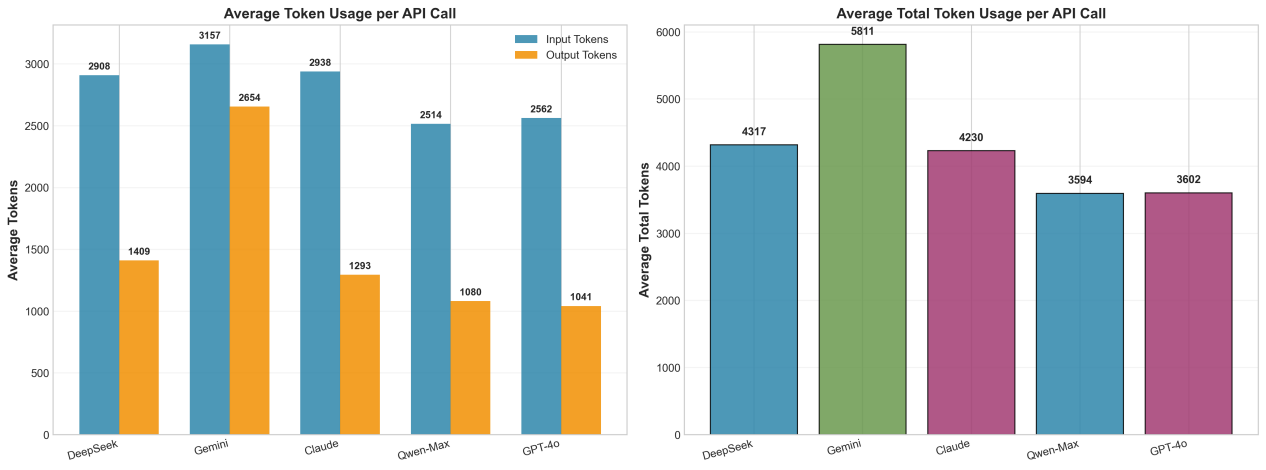
\includegraphics[width=\textwidth]{figures/media/image1.png}
\caption{Token Usage Comparison~\cite{wang_decoding_2019}.}\label{fig:token-usage}
\end{figure*}

\textbf{Fig. 1.} Token Usage Comparison~\cite{wang_decoding_2019}

Temperature is tuned to the task: lower settings support fidelity and repeatability in legal analysis, whereas higher settings encourage diversity during question generation. We use stage-specific temperatures to balance reliability and coverage: 0.3 for case answering to reduce variance, 0.7 for question generation to encourage diverse issue coverage, 0.1 for verbatim extraction to maximize fidelity, and 0.5 for comparative analysis to support richer synthesis. Top-k is left unset and API defaults are retained to avoid unnecessary interference with optimised sampling behaviour. Each question is run in a fresh chat session to prevent conversational carryover. The evaluation covers several representative model families, including GPT 4o~\cite{openai_hello_2024}, GPT 5~\cite{openai_introducing_2025}, DeepSeek R1~\cite{deepseek_deepseek-r1_nodate}, DeepSeek V3~\cite{deepseek_deepseek-v3_2025}, Qwen Max~\cite{alibaba_qwen-max_2024}, Gemini 2.5 Flash~\cite{doshi_gemini_2025}, and Claude Opus 4~\cite{anthropic_claude_2025}.

\subsection{Evaluation Rubric}\label{subsec3}

Our evaluation rubric mirrors how Chinese courts justify outcomes. It departs from common law designs that emphasize precedent selection and analogical reasoning. Chinese decisions typically start from statutes and high-level legal standards. The judge states the governing norm as the major premise.~\cite{wang_decoding_2019} The judge then maps disputed facts and issues onto that norm as the minor premise. The disposition follows as a reasoned conclusion. This deductive structure motivates our scoring. This benchmark tests whether an LLM can move from abstract norms to case-specific judgments in a disciplined way. It also examines the model's ability to exercise value-laden discretion when standards are open-textured.

\begin{figure*}[t]
\centering
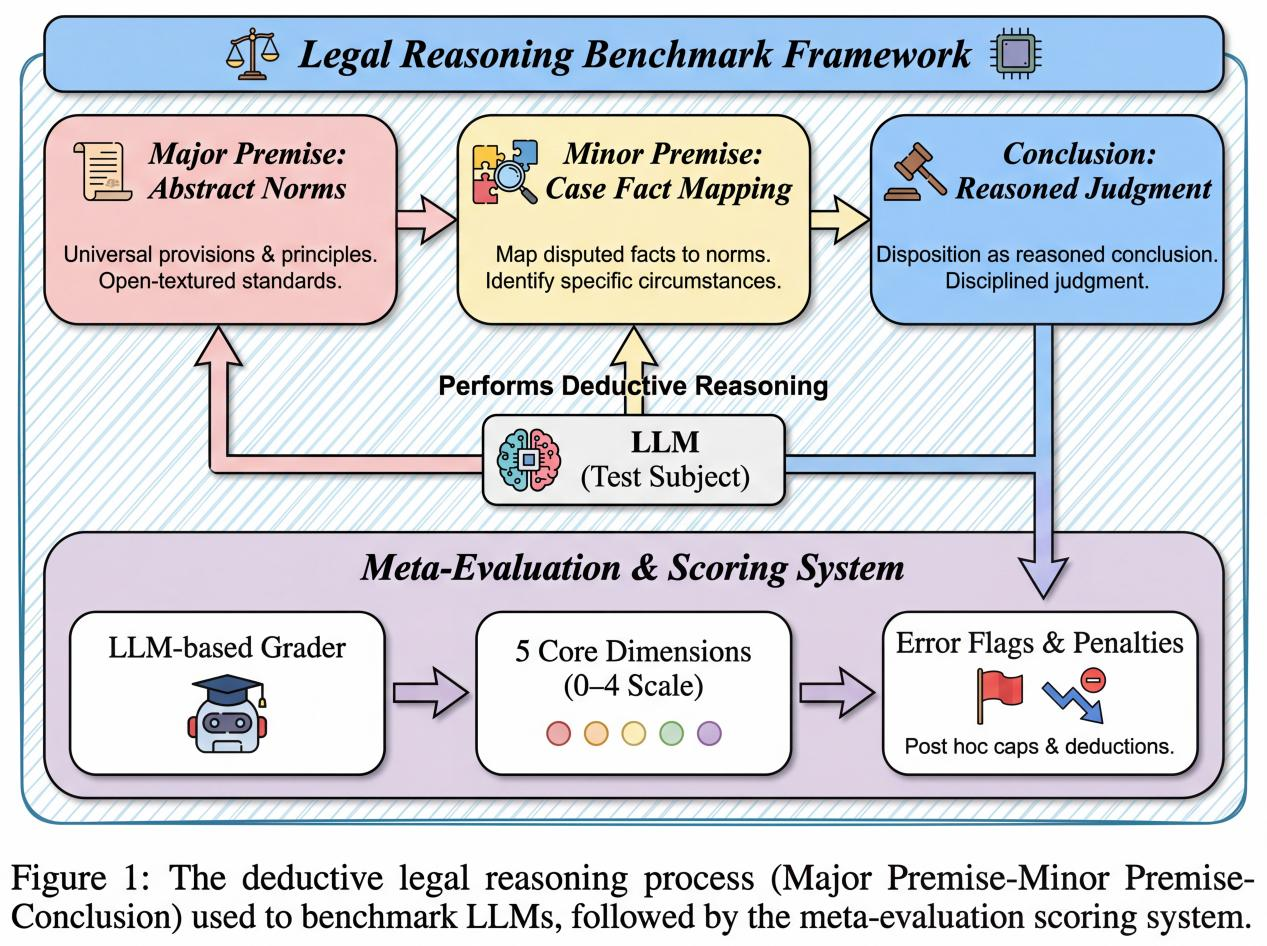
\includegraphics[width=\textwidth]{figures/media/image2.jpeg}
\caption{The deductive legal reasoning process.}\label{fig:deductive-reasoning}
\end{figure*}

\textbf{Fig. 2.} The deductive legal reasoning process

The meta-evaluation system uses an LLM-based grader to score each output on a 0--4 scale across five core dimensions. It applies impactful error flags as post hoc penalties, including score caps and deductions. The rubric uses five core dimensions plus error flags and automatic penalties.

\begin{enumerate}
\def\labelenumi{\arabic{enumi})}
\item
  \begin{quote}
  \textbf{Normative basis relevance}, i.e., is the invoked statute, interpretation, or other authority operationally relevant and accurate, rather than generic or fabricated?
  \end{quote}
\item
  \begin{quote}
  \textbf{Subsumption chain alignment}, i.e., does the answer connect issue to norm to elements or factors to facts to sub conclusions to final conclusion, without gaps?
  \end{quote}
\item
  \begin{quote}
  \textbf{Value balancing and empathy alignment}, i.e., does the answer identify the right value axes and weigh them in a restrained and professional way, without victim blaming or stigmatizing inferences?
  \end{quote}
\item
  \begin{quote}
  \textbf{Key facts and issue coverage with evidence mapping}, i.e., does the answer capture decisive facts and disputes, distinguish established versus disputed points, and tie each inference to record support without invention?
  \end{quote}
\item
  \begin{quote}
  \textbf{Outcome and remedy alignment}, i.e., is the proposed disposition and relief allocation consistent with the rule fact value chain and functionally equivalent to the reference decision?
  \end{quote}

  We evaluate a representative set of frontier LLMs spanning multiple providers and training paradigms, including both standard chat models and explicit reasoning-mode variants.~\cite{magesh_ai_2024} All systems run through the same four-stage pipeline. The case text is first masked for privacy. Dispute-centered questions are then generated from the masked record. Each model produces answers under task-adaptive temperature settings. Outputs are scored using the five-dimensional Rubric. We record impactful error flags separately. We then apply predefined caps and deductions to penalize operationally unsafe failures (e.g., fabricated authority, misreadings of core facts, and harmful value errors). Annotation proceeds at the paragraph and authority levels. Each cited authority is checked for relevance and correct use. Missing or added elements and discretionary factors are recorded, along with any fabricated source, norm, or fact. Expert scoring is costly, so a meta-evaluation task is added to test whether LLM graders can track expert judgments. We treat meta-evaluation as a complementary reliability check rather than a replacement for expert scoring. In our pipeline, meta-evaluation is used for calibration and quality control alongside the primary expert annotations. We report both the raw five-dimension totals and the penalty-adjusted scores to make the impact of error flags explicit.

\begin{figure*}[t]
\centering
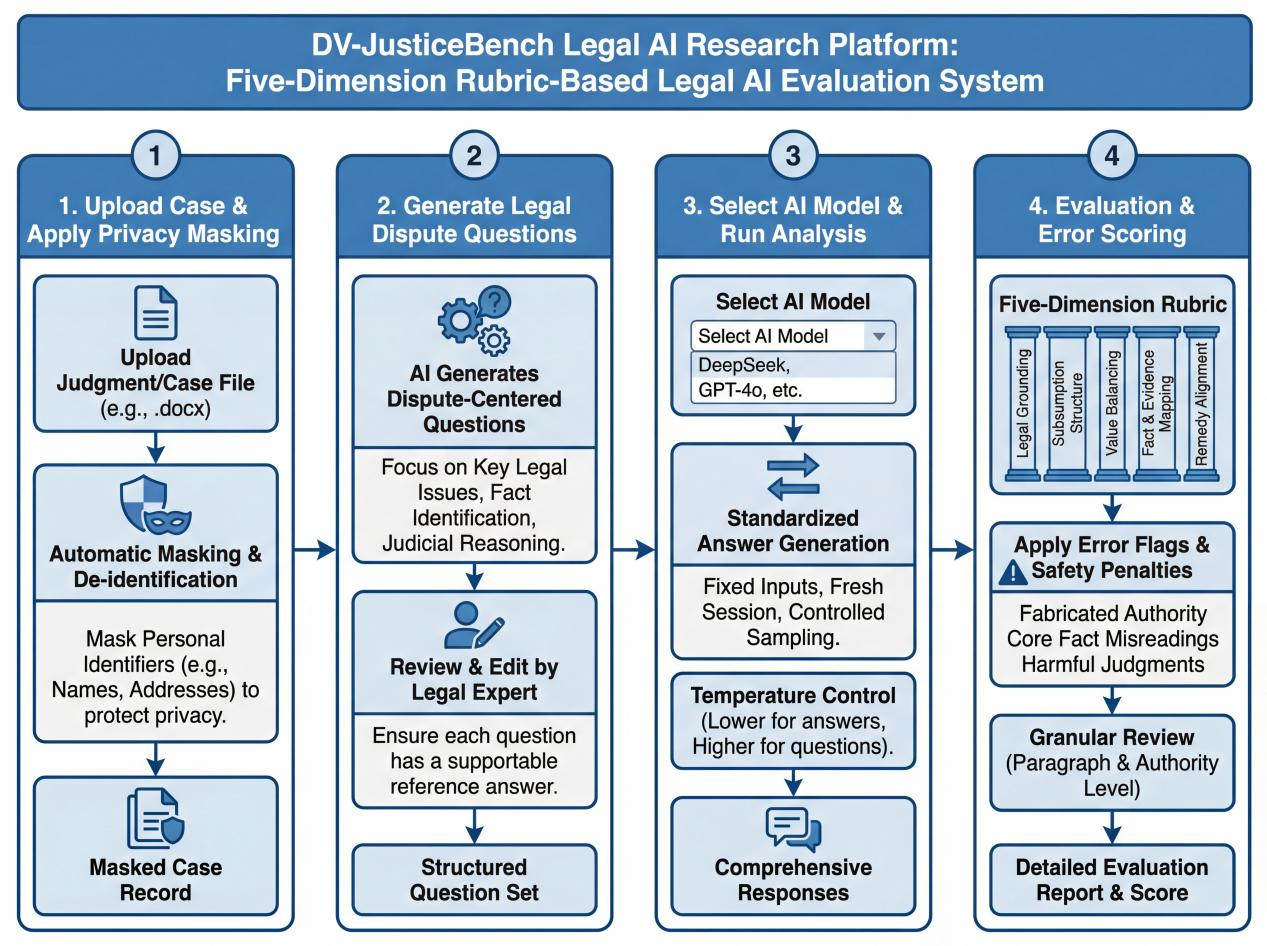
\includegraphics[width=\textwidth]{figures/media/image3.jpeg}
\caption{DV-JusticeBench workflow: a four-stage rubric-based legal AI evaluation pipeline.}\label{fig:workflow}
\end{figure*}
\end{enumerate}

\textbf{Fig. 3.} DV-JusticeBench workflow: a four-stage rubric-based legal AI evaluation pipeline

\section{Results}\label{sec4}
We report model performance in a curated, expert-vetted question set for evaluation

using three complementary lenses: (i) rubric score (primary ranking signal), (ii) reliability and error signals (failure modes not fully captured by averages), and (iii) cost/verbosity signals (token and length, where available). All metrics are produced under our four‑stage pipeline: (1) privacy masking, (2) dispute‑centered question generation (expert‑reviewed), (3) standardized answer generation (fixed system prompt, stable input order, fresh sessions to prevent carryover), and (4) rubric scoring with authority‑level auditing cues. Cohen's Kappa was calculated for each dimension: Normative Basis Relevance ($\kappa$= 0.85), Subsumption Chain Alignment ($\kappa$= 0.83), Value Balancing \& Empathy ($\kappa$= 0.72), Key Fact Coverage ($\kappa$= 0.86), and Outcome Consistency ($\kappa$= 0.84). The lower agreement on Value Balancing reflects the inherent subjectivity of empathy assessment, while the high consistency on objective dimensions (Normative Basis, Key Facts) validates the clarity of our rubric. The overall weighted Kappa was 0.82, indicating substantial agreement.

\begin{figure*}[t]
\centering
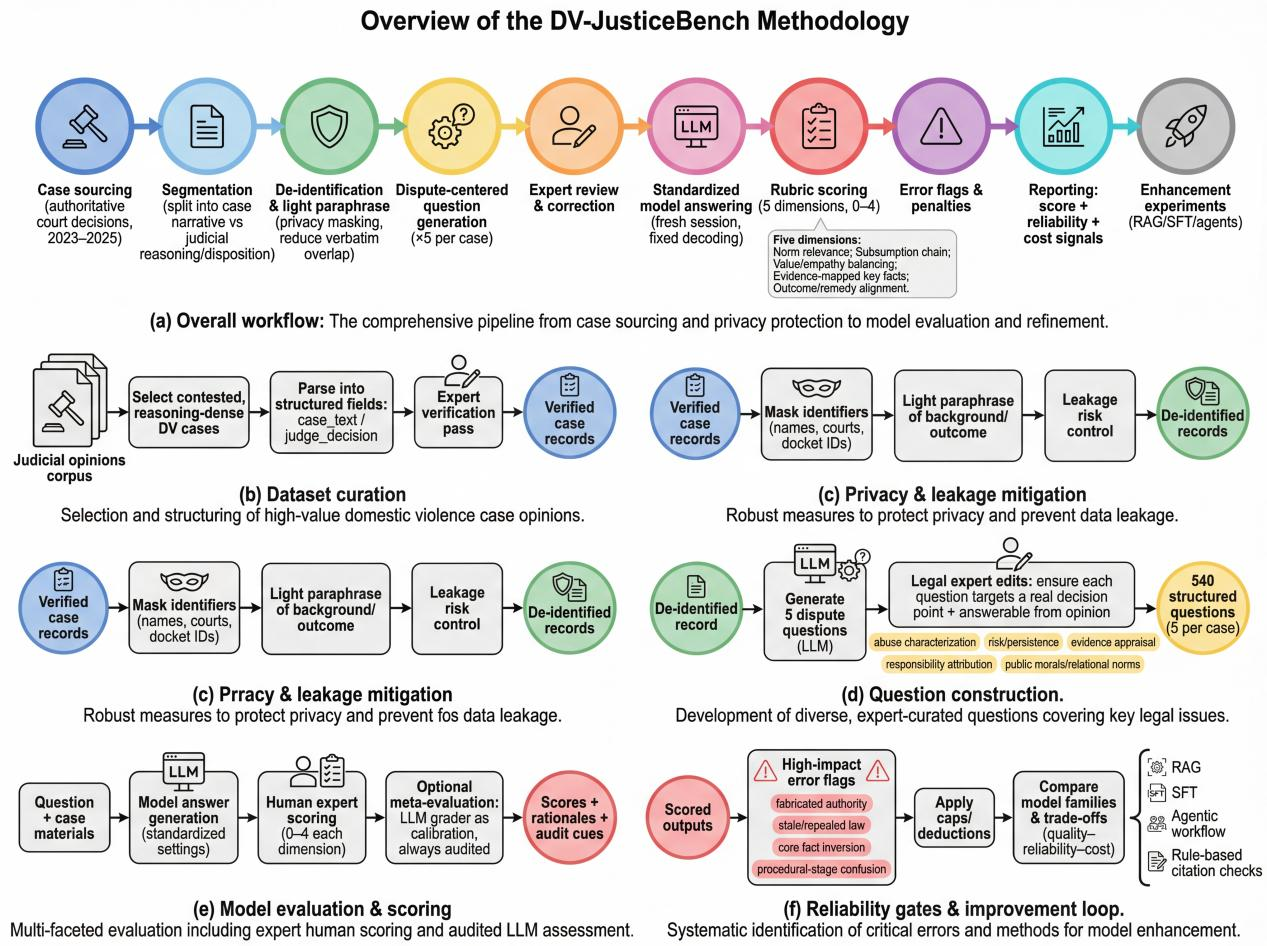
\includegraphics[width=\textwidth]{figures/media/image4.jpeg}
\caption{End-to-End Methodology and Evaluation Pipeline.}\label{fig:methodology}
\end{figure*}

\textbf{Fig. 4.} End-to-End Methodology and Evaluation Pipeline

\textbf{Score-based ranking.} Figure 1 ranks models by the mean total score (out of 20), aggregated from the five 0--4 rubric dimensions, with impactful-error flags applied as post-scoring penalties. The ordering is: DeepSeek‑Thinking (16.45), DeepSeek (16.42), Gemini (15.63), Claude (13.11), Qwen‑Max (10.36), and GPT‑4o (9.39). The separation is driven primarily by alignment with judicial reasoning and evidential discipline, not by writing style. Dimension (Fig.4) means show the steepest drop from the top tier to GPT‑4o in Subsumption Chain Alignment (3.39 vs. 1.71) and Key Facts/Issues Coverage (3.25 vs. 1.68), which explains why lower-ranked models can sound plausible yet fail to reproduce the court's norm‑to‑fact proof structure.

\begin{figure*}[t]
\centering
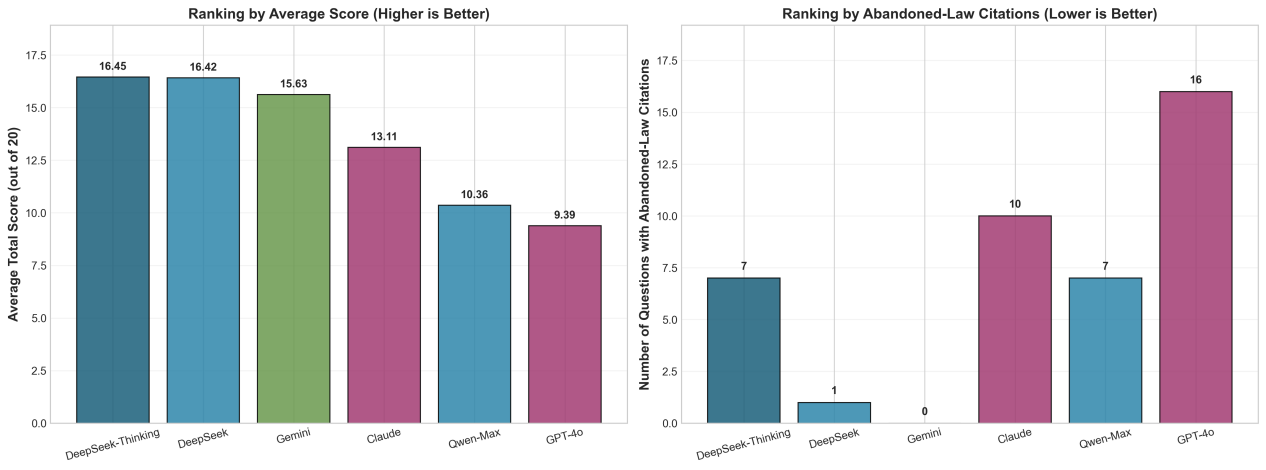
\includegraphics[width=\textwidth]{figures/media/image5.png}
\caption{Overall Ranking.\protect\footnote{Figure 5 summarizes the final ranking: (1) DeepSeek-Thinking, (2) DeepSeek, (3) Gemini, (4) Claude, (5) Qwen-Max, (6) GPT-4o. The top two are statistically tied, and the gap between tiers is substantial.}}\label{fig:overall-ranking}
\end{figure*}

\begin{figure*}[t]
\centering
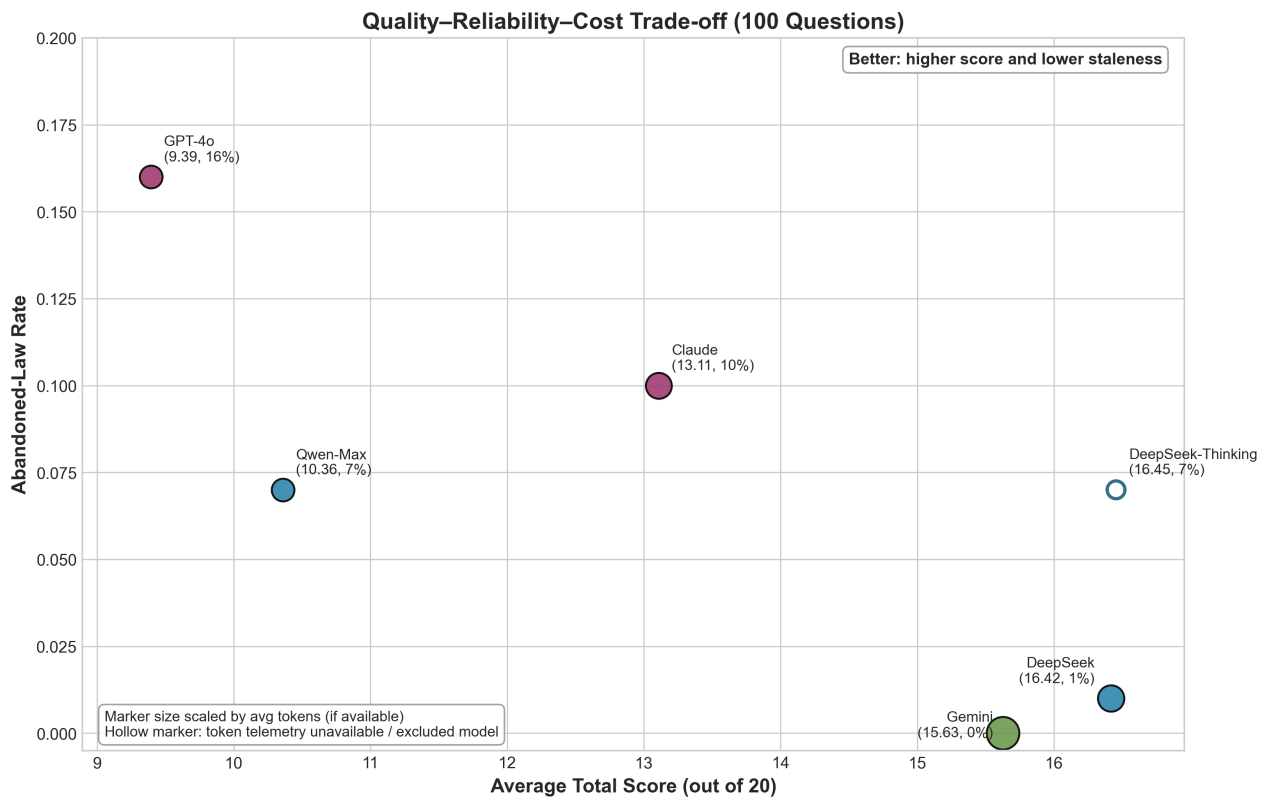
\includegraphics[width=\textwidth]{figures/media/image6.png}
\caption{Pareto Trade-off (Quality--Reliability--Cost).\protect\footnote{To synthesize quality, reliability, and efficiency into a single view, we construct a Pareto frontier plot (Figure~6) with three dimensions: (i) rubric score (y-axis, 0--20), (ii) reliability measured as the inverse of abandoned-law citation rate (x-axis, where higher = more reliable), and (iii) computational cost encoded as bubble size (average total tokens per question). Models on or near the upper-right frontier represent better trade-offs. DeepSeek achieves the highest reliability score (1.0 inverse rate, only 1/100 abandoned citations) with a mean score of 16.42/20 and moderate token usage (avg.\ 4,247 total tokens), placing it at the efficiency frontier. DeepSeek-Thinking adds +0.03 points (16.45/20) at slightly higher cost (avg.\ 5,038 tokens) and lower reliability (7/100 abandoned), illustrating a score-reliability tradeoff within the same model family. Gemini matches DeepSeek's reliability (0/100 abandoned) but scores lower (15.63/20) and consumes fewer tokens (avg.\ 3,126), occupying a different region of the frontier. Claude, Qwen-Max, and GPT-4o fall below the frontier, with GPT-4o exhibiting both the lowest score (9.39/20) and the highest abandoned-law rate (16/100). This analysis confirms that no model dominates all three dimensions simultaneously, and deployment decisions must weigh score gains against reliability risks and cost constraints.}}\label{fig:pareto-tradeoff}
\end{figure*}

\subsection{Model Performance Heatmap}\label{chart_heatmap_dimensions_20260118_222455}
\begin{figure*}[t]
\centering
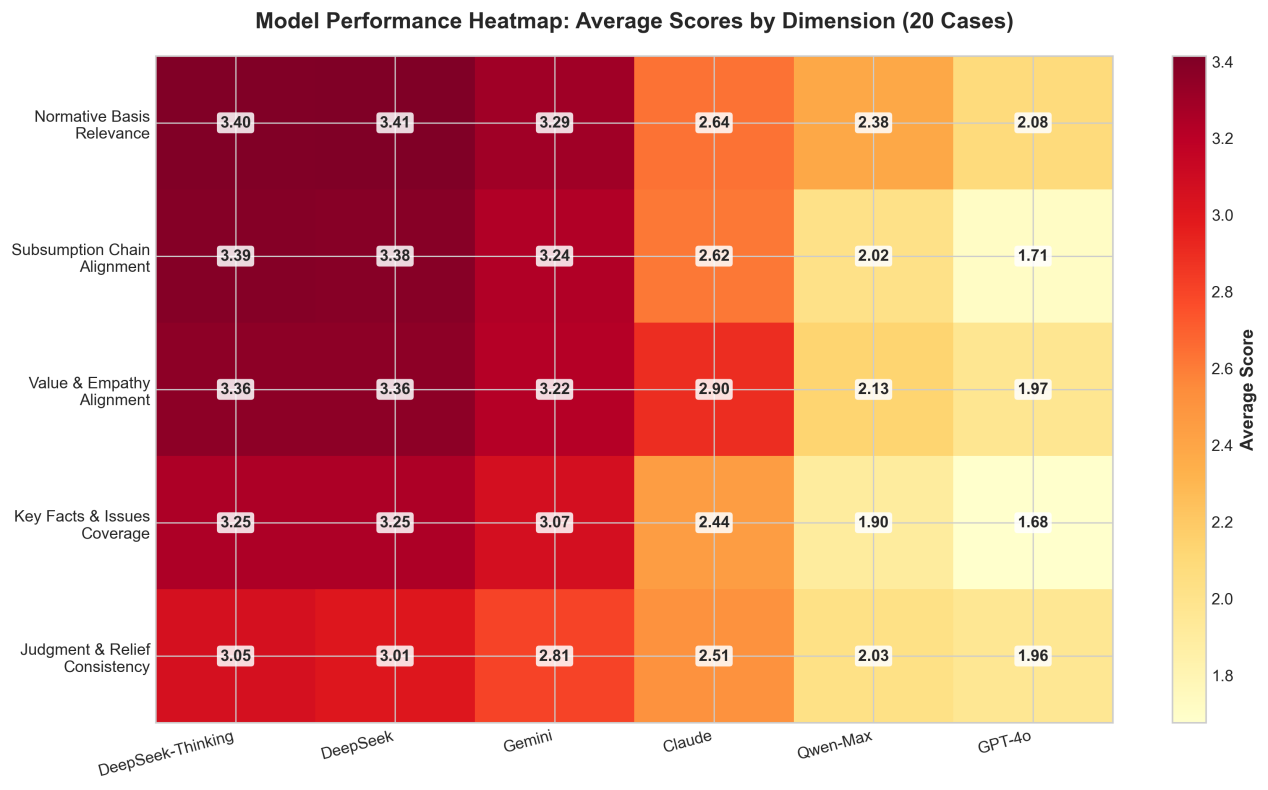
\includegraphics[width=\textwidth]{figures/media/image7.png}
\caption{Model Performance Heatmap: Average Scores by Dimension.\protect\footnote{Figure 7 decomposes scores into five rubric dimensions. Top-tier models excel in Subsumption Chain Alignment (3.39--3.42/4) and Key Facts Coverage (3.25--3.30/4), while lower-ranked models show steepest drops in these two dimensions. Value Balancing remains challenging across all models (range: 2.29--3.28/4).}}\label{fig:heatmap-dimensions}
\end{figure*}

\textbf{Fig. 7.} Model Performance Heatmap: Average Scores by Dimension~\cite{magesh_ai_2024}

\textbf{Error profiles explain rank differences.} Counts of high-salience errors co-vary with score. Qwen‑Max has the most major errors (4) and a high obvious-error load (78). GPT‑4o has the highest count of obvious errors (86). By contrast, DeepSeek‑Thinking and DeepSeek have far fewer obvious errors (29 and 31), consistent with stronger subsumption and fact‑mapping behavior.

\begin{figure*}[t]
\centering
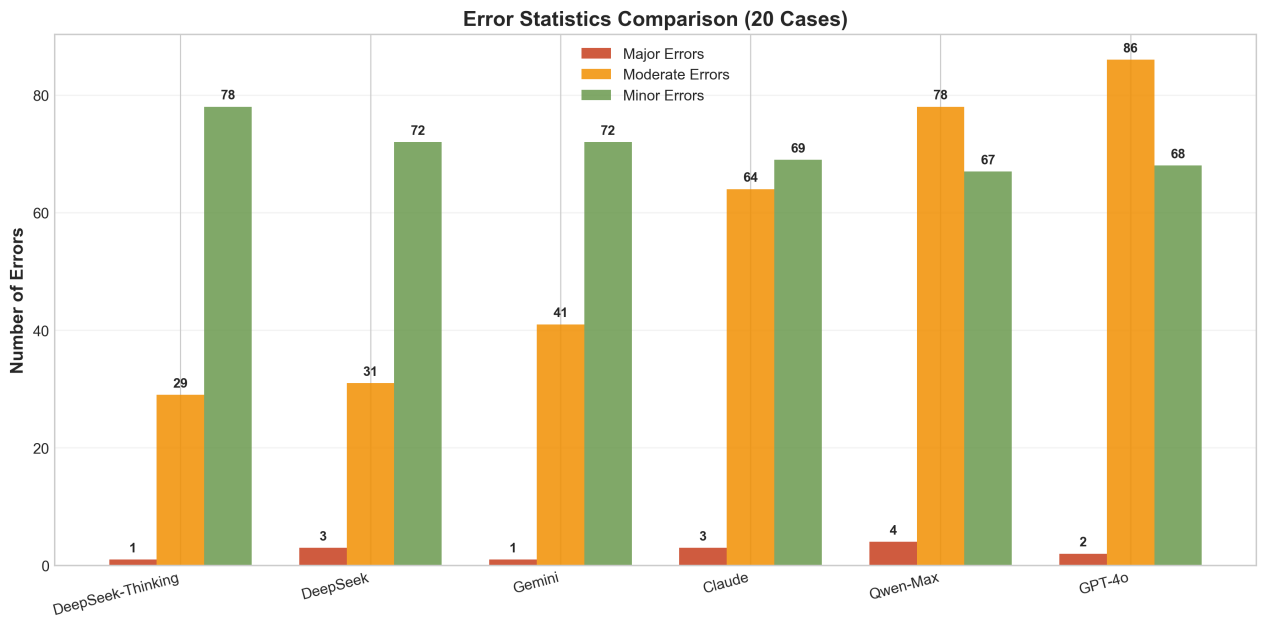
\includegraphics[width=\textwidth]{figures/media/image8.png}
\caption{Error Statistics (Major/Obvious/Minor).}\label{fig:error-stats}
\end{figure*}

\textbf{Why we report reliability signals alongside ranks.} Average score can mask operational risks. We therefore report abandoned-law citations as a concrete reliability signal: 0/100 for Gemini, 1/100 for DeepSeek, 7/100 for DeepSeek‑Thinking, 7/100 for Qwen‑Max, 10/100 for Claude, and 16/100 for GPT‑4o. This matters because an answer can be fluent and empathetic yet unusable if it relies on repealed authority. Notably, DeepSeek‑Thinking yields only a +0.04/20 gain over DeepSeek on average score (16.45 vs. 16.42) but increases abandoned-law citations (7 vs. 1), highlighting a score--reliability trade-off relevant to deployment.

\textbf{Cost and verbosity signals} (where token telemetry is available). In the answer-generation stage, average total tokens per response range from 3,594 (Qwen‑Max) to 5,811 (Gemini), with DeepSeek at 4,317 and Claude at 4,230 (token telemetry is not uniformly available for all models). Output verbosity also varies substantially: average answer length ranges from 1,060 characters (GPT‑4o) and 1,357 (Qwen‑Max) to 3,773 (DeepSeek) and 3,888 (Gemini). These signals show that longer outputs and higher token usage do not guarantee higher judicial alignment, and they support reporting quality together with compute cost for practical selection.

\textbf{Why impactful errors are penalties rather than a sixth dimension.} We treat fabricated authority, core fact inversion, and procedural-stage confusion as high-impact failures that should cap or deduct scores across dimensions. This prevents double-counting while keeping the primary ranking anchored to the five judicial-quality dimensions.

\textbf{Handling GPT‑5.} We exclude GPT‑5 from the main ranking because content-sensitivity constraints led it to refuse answers for a majority of prompts in this slice (65/100). We report it separately: among the 35 non-refused responses, the mean score is 16.60/20, but the refusal behavior makes cross-model ranking less comparable in this setting.

Overall, the gap between tiers is explained by both aggregate scores and error profiles. Models with weaker subsumption-chain alignment and key-fact/issue coverage accrue more high-salience errors, which can yield fluent but court-misaligned outputs. As Figure 1 suggests, top-tier models are consistently strong across the rubric dimensions rather than spiking in a single component.

Figure 6 summarizes abandoned-law citations as a reliability indicator and highlights a within-family trade-off: the reasoning mode yields marginal score gains while increasing stale-law risk.

\section{Discussion}\label{sec5}
The results above show where models perform well and where they break down.\\
We now move to text-level analysis to explain these patterns and illustrate how reasoning succeeds or fails in practice.

\subsection{Judicial Reasoning Alignment}\label{subsec5}
\textbf{Normative Basis Relevance.} Dimension-level averages in the 100-question slice show a consistent gradient: DeepSeek‑Thinking and DeepSeek score \textasciitilde3.4/4 on Normative Basis and Subsumption, while GPT‑4o is \textasciitilde2.1/4 on Normative Basis and \textasciitilde1.7/4 on Subsumption; the largest gaps concentrate in Key Facts/Issues Coverage (3.25 vs. 1.68) and Subsumption (3.39 vs. 1.71). Normative basis relevance measures whether a model selects rules that actually do work in the case. It tests ``operational relevance,'' not general legal education. In a statute-centered civil law setting, the governing norm functions as the major premise. When the rule is wrong, later subsumption can look fluent but stays ungrounded. The point is not whether the model reaches the ``right'' outcome. The point is whether the cited authority supports elements, exceptions, or discretionary factors as courts use them. In domestic violence characterization, DeepSeek and Gemini often start from the definition clause in the Anti-domestic Violence Law of the PRC, including `` the inflicting of physical, psychological or other harm...'' In custody and protection-order disputes, higher scoring answers cite both the child-centered standards in the Civil Code art. 1084, ``best interests of the minor'' and art. 1085, support payments and the protection-order gateway norms ( Anti-domestic Violence Law, arts. 23 and 27, ``personal safety protective order'' ). In divorce, property, and damages, Qwen-Max and Gemini are most reliable when they map each claim to the corresponding article, such as divorce grounds, property division, housework compensation, and divorce damages. In homicide cases triggered by long-term abuse, DeepSeek's better answers separate conviction from sentencing and cite the crime definition and voluntarily giving oneself up (Criminal Law of the PRC, art. 232 and art. 67). One representative answer makes the sentencing move explicit: ``recommend a substantial mitigation within the sentencing range for intentional homicide, but not a downward adjustment to the next range.'' This citation pattern matches what judges treat as legally ``actionable'' in their written reasons.

Besides, failure cases are rarely random. They reflect a structural gap between model citation habits and judicial discretion. A common miss is slogan-level reliance on broad principles. DeepSeek sometimes frames disputes with the Civil Code art. 8 ``public order and good morals'' and art. 153 ``void juridical act.'', yet it does not connect them to the court's operative tool, such as intent-interpretation rules in a waiver or settlement setting. One typical phrasing is: ``legal protection of personal rights is the cornerstone of social order,'' which sounds normatively appealing but can miss the judge's technical path. Another recurring weakness is thin procedure and evidence law. Complex fact patterns often turn on burden allocation and proof rules under the Civil Procedure Law, including the baseline ``who asserts, who proves'', yet many LLM answers stay on entity law only. Norm mixing is another source of low scores. Qwen-Max occasionally cites the marital community-property rule in a cohabitation case (Civil Code of the PRC, art. 1062 ``community property and ...joint possession''), then tries to walk it back. That starting point still distorts the legal frame. Claude sometimes omits the decisive gift rule when ``gift'' is the disputed label (Civil Code of the PRC, art. 657 ``gift contract'').

Update lag is measurable in our slice via abandoned-law citations: Gemini has 0/100 (0.0\%), DeepSeek has 1/100 (1.0\%), DeepSeek‑Thinking and Qwen‑Max each have 7/100 (7.0\%), Claude has 10/100 (10.0\%), and GPT‑4o reaches 16/100 (16.0\%). For bride price disputes, answers that cite older interpretive anchors instead of the newer SPC bride price provisions lose ``operational'' precision (Provisions by the Supreme People's Court on Several Issues Concerning the Application of Law in the Trial of Cases Involving Betrothal Gift Disputes, arts. 5--6). Finally, some judgments draw on international norms to signal a protective orientation. Models rarely mirror that layer, such as CEDAW-related guidance (The Convention on the Elimination of all Forms of Discrimination Against Women), which reduces completeness when the decision itself uses it as a legitimating frame.

These patterns explain why normative basis relevance is a structural marker of judicial alignment. It is also a legitimacy proxy. Public acceptance of AI legal support can be high, even when it is explicitly non-human.~\cite{flanagan_rule_2025} In this benchmark, high scores come from disciplined rule selection and function-aware citation. Low scores come from generic principles, domain mismatches, missing procedural anchors, and stale or omitted controlling sources.

\textbf{Subsumption Chain Alignment.} The strongest outputs treated legal labels as propositions to be proven, then forced them through factorization and mapping. DeepSeek did this well in a domestic violence framing task. It began with the dispute issue, whether the victim's conduct is better characterized as improper provocation or domestic violence, as the victim's fault. It then stated a norm under the Anti-domestic Violence Law, art. 2. It broke ``domestic violence in the legal sense'' into three working parts, such as a control like a harmful act, a causal link to the offense, and a proportionality threshold tied to urgent safety risk. It then mapped concrete facts into each part, including long-term verbal abuse and control, property destruction at the scene, a slap, and the knife stabbing directed at a sofa. It marked key items as not satisfied with reasons that track a judge's review logic, such as the knife act targeting property, the record not supporting homicidal intent, and the sequence looking like retaliation rather than a direct response. The sub-conclusion, not domestic violence in the legal sense, followed from those itemized judgments rather than from rhetoric.

The same disciplined structure appeared when models used court-like sequencing in defense and protective relief contexts. DeepSeek often used the recognizable two-stage path for legitimate defense: whether legitimate defense is established, and, if so, whether it is excessive. It operationalized Guiding Opinions, art. 10, as testable factors. It tied factors to specific record facts, such as a large power gap, one successful knife seizure, a later sequence of 17 stabs, and post-event statements, and it explained why each factor was met or not met before issuing a sub-conclusion. Gemini showed parallel strength in protection order cases by linking the Anti-domestic Violence Law, art. 2, and art. 23 to a structured, realistic danger analysis. It did not stop at "there is danger." It broke down danger into record, facing risk factors, then grounded them in facts such as self-harm with a knife, reflecting escalation, pushing the applicant down, causing injury, reflecting direct physical intrusion, and repeated conflict, reflecting recurrence. Custody disputes showed the same pattern when Qwen and GPT operationalized the Civil Code of the PRC, art. 1084~through factors like stability, caregiving history, the child's expressed preference, parental conditions, and conduct risk, and then anchored each factor in adjudicated facts such as long-term residence with the mother and schooling near the mother's home. Remedy analysis also aligned better when Qwen separated claims into distinct sub-chains and tied each to its own norm, including divorce under Civil Code art. 1079, property division and homemaker compensation under art. 1087 and art. 1088, and damages under art. 1091.

Weaker outputs clustered around a few recurring failure types. First is norm drift or value substitution. In the settlement waiver example, DeepSeek relied on "public order and good morals" as the main engine. However, the judge's operative path focused on intent interpretation through text, context, and a sequence of acts, including the written "no pursuit" statement, the parties' failure to divorce at the time, the presence of a child, and later reaffirmation in divorce mediation. When the model swaps the court's working norm for a higher-level principle, its element mapping no longer aligns, even if the bottom line remains the same. Second is the element omission around mental violence and control. Several answers treated self-harm threats as simple knife threats, without breaking mental coercion into fear induction, control purpose, and intrusion on mental peace, which is often the judge's internal route. Third is issue drift. One Qwen chain pivoted to the victim's legitimate defense and cited the Criminal Law of the PRC, art. 20, then concluded that there was no victim responsibility. However, the dispute issue was the alleged abuser's responsibility and whether the self-harm threat supports protection order relief under the Anti domestic Violence Law art. 2 and art. 23. A closed chain that answers the wrong question is still misaligned. Finally, we also saw thin mapping~where models listed the right factors but did not perform itemized satisfaction judgments against the appellant's key defenses, as in some bride price disputes citing Civil Code art. 1042 and SPC Interpretation I art. 5 and art. 31. The factor list appears complete, yet it omits the rebuttal-driven steps courts use to justify disposition.

\subsection{Explanatory Quality and Legal Application}\label{subsec5}

\textbf{Key Facts and Issue Coverage.} A legally usable output has to do three things at the same time. It must identify the facts that truly drive the outcome, connect those facts to the relevant legal elements or discretionary factors, and maintain strict evidential discipline. The goal is to control fact status. DeepSeek performed well in the self-defense style dispute. It captured the long-term conflict background, including frequent insults and slaps, economic pressure, and social isolation. It then tracked the incident day escalation, including property damage, the police call, renewed quarrel after return, "stabbing the sofa," the verbal trigger "you should die," and the struggle into the corridor. It also captured the defendant's conduct, "seizing the knife" and "stabbing 17 times," plus physical asymmetry between the parties. The strength lay in disciplined linkage, not storytelling. DeepSeek treated "stabbing the sofa" as a legally relevant fact for intensity or immediacy, and treated long-term insults and control as inputs to the evaluation of infringement intensity and control-related factors. A second strong~example refined the same method by isolating a decisive micro fact and stating its doctrinal consequence. It stressed that "all evidence indicates the knife's direction was toward the sofa, not the defendant's body," then placed that fact into a structured frame tied to unlawfulness intensity, imminence, necessity, and intent transformation. This is a record-based legal application; the facts serve as inputs to tests.

On one hand, Strong performance also appeared in family cases when outputs treated the judgment as a proof structure.~DeepSeek did this in a divorce reasoning example by covering marriage duration, children, procedural history, and the claimed grounds such as emotional breakdown, domestic violence, rape related history, and separation, while separating what the court treated as established, such as a rape conviction history, from what remained disputed or unproven, such as continuing domestic violence or persistent separation, and mapping these into the breakdown factors and discretionary balancing the court actually used. In a protection order setting, Claude performed strongly by capturing the parties' relationship, the victim's economic dependence as a full-time homemaker, repeated domestic violence, and that the last incident had police involvement and medical proof, then mapping violence facts to the legal recognition of domestic violence and mapping economic dependence to its distinct legal relevance for compensation and responsibility. In custody modification and protection contexts, Qwen performed well when it captured the custody background, the father's long term absence for work, the child's living arrangement with grandmother and uncle, the harm facts including beatings and risk of sexual abuse, and the evidence anchors like injury appraisal and the child's letters, then mapped those facts into protective duties under the Anti-domestic Violence Law and the Law of the People's Republic of China on the Protection of Minors (2024 Amendment). Gemini also performed well in another domestic violence context by clearly separating the parties' assertions from the court's findings. It treated the workplace "slap" incident and the supporting materials as evidence to be weighed, while correctly noting that the trial court's domestic violence finding was affirmed on appeal, and then mapping those facts to the legally relevant violence and proof structure.

On the other hand, weak outputs cluster into repeatable legal failure types.~Evidential defaulting appears when an answer treats one side's story as proven. In one case, DeepSeek built its analysis almost entirely on the applicant's asserted facts and evidence, implicitly assuming that chat logs and injury photos proved the claim. The court's decisive point was the opposite, and the evidence "could not achieve the purpose of proof." Because that dispositive evidential status was omitted, the later Subsumption became a doctrine applied to an imagined record. A related inference inflation shows up in Claude, which introduced "economic control" as a case fact even though the materials did not establish restrictions on economic autonomy, reasoning instead from "common patterns" and financial context. Another failure is that facts are listed but assigned the wrong legal meaning. In a protection order dispute, Claude captured "self-harm threats with a knife" and "pushing leading to injury," yet reframed the case as bodily harm and failed to treat the knife-based self-harm threat as the decisive act for psychological violence. The judgment's core was that the husband did not directly beat the wife, but the knife threat caused fear and constituted psychological violence. GPT showed a parallel mapping weakness by capturing the knife threat and injury, but underemphasizing the separate psychological fear, finding that the judgment was treated as an independent basis for domestic violence recognition.

Focus drift is also common. In an appellate custody case, GPT focused on domestic violence recognition and imported facts like slapping and evidence media, even though the appellate court had already confirmed domestic violence and set the only live issue as custody allocation. GPT then failed to cover the decisive custody facts, including that the children had lived with the mother for nearly three years after separation, attended school near the maternal family with a stable environment, the court asked the daughter's preference, and she wanted to live with the mother. Geographic distance would impose major environmental change costs. A parallel drift pattern appeared in Gemini, where the answer accurately summarized domestic violence facts but still analyzed whether domestic violence was established, even though the appellate decision framed custody as the only live dispute. In a separate case, Gemini's fact summary was directionally right. However, it showed a minor timeline imprecision, treating "formal case filing" as occurring before an asset transfer, even though the record sequence was tighter.

Besides, procedural posture omissions are uniquely damaging. This appeared in DeepSeek in retrial-review contexts, where the output summarized the applicant's retrial claims and mapped them into substantive elements, but omitted that the applicant did not appeal within the statutory period without justification and that the applicant provided no new evidence in retrial review. Similar "missing the dispositive factor" problems appeared in Qwen in a betrothal gift return dispute, where the answer captured the gift amount and short cohabitation but omitted contested fault allegations, such as domestic violence and lack of support during miscarriage, that the court used to set the return ratio. It also omitted the woman's new appellate request about a gold ring. Another example is Qwen in a funds dispute, where the output captured transfers but over-emphasized the "improper relationship" and failed to integrate the offsets and net difference calculation system the court actually used, even though that calculation was the core basis for the "no legal basis" reasoning. These are not missing details. They are missing the facts that drive the legal conclusion.

\textbf{Outcome and Remedy Alignment.} LLM outputs may look more stable than human decisions because they lack intrinsic human variability.~\cite{zanotto_human_2024} Yet stability is not the same as legal alignment, especially when the remedy is multi-layer and operational. Several outputs showed high-quality alignment. Although~in some homicide cases, DS tracked the court's direction and its sentencing logic. It agreed with rejecting a domestic violence finding, while still treating the victim's role in escalation as relevant mitigation. It treated confession as a key leniency factor. Functionally, that matched a life imprisonment disposition and signaled severe punishment calibrated by mitigation. DS also aligned its aggravating factors, such as brutality and severe consequences, and its mitigating factors, such as surrender, remorse, victim contribution, family conflict trigger, and compensation and forgiveness, with the court's actual considerations.~DS also aligned well when the remedy structure was hybrid and task-specific, not purely monetary. In a case involving both a personal safety protection order and a custody change, DS recommended the immediate issuance of a protection order and included standard prohibitions, such as no violence, no harassment, and no contact, plus a move-out measure tied to cohabitation risk. The court issued a six-month prohibition package. The core relief, a strong no-contact prohibition regime, was functionally equivalent.

Monetary relief alignment was also strong, where models kept remedy components tied to proven losses and legal duties. DS explicitly supported the court's economic compensation items, such as medical expenses, lost wages, nutrition, nursing, and property loss, and it supported non-economic accountability, such as apology, while treating the calculation and allocation as reasonable. The structure mattered more than precision. The model endorsed the same categories of relief and justified them through its own prior legal analysis without internal conflict. In divorce and domestic violence settings, Claude showed strong outcome and remedy type alignment. It endorsed granting divorce, recognizing domestic violence, tilting property division toward the victim, awarding divorce damages, and awarding domestic labor compensation. It did not provide a numerical split, but it aligned with the court on the remedy architecture. In marital debt litigation with a domestic violence context, GPT's remedy suggestions, such as re-examining debt character, accounting for the domestic violence context, and placing the burden on the creditor, were functionally aligned with remand or reversal paths.~

In a custody change case, Qwen matched the direction and the key relief allocation. It recognized domestic violence, supported custody change to the mother, and treated continued protection order enforcement as necessary. It also linked child mental health to relief design by recommending counseling and treatment, matching the court's emphasis that the father failed to address the child's diagnosis and caused secondary harm. Gemini matched the direction by recognizing domestic violence, rejecting victim responsibility, and supporting protective orders. It then proposed a set of linked measures, including strict enforcement of protection orders, civil compensation, divorce litigation, assessment of criminal liability, attention to children, and perpetrator intervention. The court's remedy path was operational and multi-agency, including service and warning, coordinated monitoring and support, fines and admonition, shelter provision, mediated divorce, and attention to minors' mental health. Gemini's package was functionally equivalent in purpose and structure, as both implement a layered response that moves from immediate protection to accountability and to longer-term stabilization.

However, misalignment often shows up in the remedy layer even when the overall direction is plausible. In the homicide case, DS sometimes predicted sentences of death with a two-year suspension of~execution rather than life imprisonment. Both reject immediate execution and sit within a realistic sentencing range, but they are not the same legal form. The difference matters because they diverge in legal status, execution mechanics, and later commutation pathways. Importantly, DS's own mitigation chain pointed toward leniency.~A recurring weakness is the thinness of remedies in cases where the court's relief is a system rather than a single order. In a protection order case, Claude aligned with issuing the protection order, but did not reflect the court's closed-loop design. The court paired issuance with service and warning, multi-agency coordination, ongoing monitoring, sanctions for violations such as fines, and shelter support. Claude largely stopped at rapid issuance and did not integrate enforcement, supervision, consequences for violations, or coordinated protection for victims and minors. The direction was right, but the remedy was not functionally equivalent to what the court actually built. The same thinness appeared in GPT. In one protection order setting, GPT supported maintaining the order and suggested mediation and monitoring. However, it did not align with the court's layered mechanism, which included fines, admonition, shelter provision, and child-focused measures that ultimately supported a mediated divorce. This gap is practical, not stylistic, because it changes how the remedy operates.

Remedy drift also occurs when issue drift prevents the model from landing on the court's decisive allocation. In an appellate custody dispute, Claude offered a defensible sub view that a single physical friction episode may not, by itself, constitute legal domestic violence. That stance was not necessarily inconsistent with the court, because the court did not treat domestic violence as the deciding factor. The failure was at the remedy endpoint. The court's key relief was the allocation of custody, which it affirmed in favor of the mother based on stability and welfare factors. Claude's remedy section remained abstract and did not yield a clear custody allocation that matched either its reasoning or the court's disposition. This captures the core risk in this dimension. Legal characterization alone is not enough unless it translates into a concrete relief allocation.

More serious misalignment appears as outcome reversal, where the proposed remedy architecture conflicts with the reference judgment direction. In property division, DS treated domestic violence as the central driver and proposed a materially greater-than-half share for the wife, with concrete adjustments, such as using the actual sale price for an office building, sharply tilting housing proceeds, and scrutinizing equity transfers. The court did the opposite. It dismissed the appeal and maintained the equal division, citing procedural limitations and rejecting the appellant's arguments. DS's chain may be coherent in isolation, but it fails to align in direction and relief with the reference. Reversal risks are amplified in retrial and rehearing contexts, where the remedy question is often procedural before it is substantive. Qwen recommended rehearing and implied the original judgment was wrong, while the court dismissed the rehearing application. A similar reversal occurred when DS proposed revising the judgment to support damages for mental distress. At the same time, the court dismissed the rehearing for insufficient evidence and the absence of an appeal or new evidence. In these settings, remedy alignment depends on procedural posture. If a model overlooks or discounts procedural bars, it can generate a coherent substantive package that still conflicts with the adjudicative path the court legally must follow.

Another recurring weakness is over-weighting a factor that the court treated as one circumstance among many. In a betrothal gift return dispute, Gemini argued that conduct should be explicitly labeled as domestic violence and used as a major lever to change the return amount. The court treated the injury event as one factor among others in a broader balancing test and still set a high return ratio. Gemini's proposed relief structure elevated domestic violence into a decisive adjustment, which was not functionally equivalent to the court's balancing design, even if the moral intuition was understandable.~Where the remedy is relatively simple and the record points to a clear endpoint, such as granting divorce, changing custody, or excluding a debt from marital liability, LLMs often track the correct direction and core relief categories. Where relief is multi-layer, operational, or procedurally constrained, alignment becomes fragile.

\subsection{Value-laden Decisions}\label{subsec5}
Unlike math or logic tasks, where conclusions follow from facts, judicial writing often turns on normatively charged and open-textured terms such as reasonable, substantial emotional distress, or ambiguous statutory language that admits multiple readings.~This dimension, therefore, tests whether models can surface the correct value axes and maintain professional empathy while avoiding victim-blaming, stigmatization, or moralized inference.~Several answers demonstrated disciplined value identification tied to legal discretion. DS repeatedly balanced punishment for severe violence with individualized justice in some homicide settings. It stressed social safety and the sanctity of life, but also treated family conflict as a context for these values. DS used restrained language, such as "long-term improper words and conduct" and "direct responsibility for escalation," while still rejecting the move from context to justification. It also separated "victim responsibility" from the legal predicates of self-defense, which reduced the risk that empathy becomes a back door to rationalizing violence. In the self-defense style dispute, DS framed the value boundary as encouraging legitimate defense while preventing abuse. That framing matters because it preserves the integrity of the defense while remaining sensitive to escalation risk. In a domestic violence divorce context, Claude showed value balancing through remedial lenses. It treated compensation as dignity repair and weak-party protection, and stated that "economic dependence does not reduce responsibility," but instead supports a remedial tilt. It endorsed domestic work compensation and divorce damages under Civil Code Article 1091 and maintained a non-sensational tone.~

In child-related cases, several models operationalize "best interests" into concrete risk and welfare factors (safety, stability, caregiving history, and mental health), and the stronger outputs keep the value discussion tethered to legally actionable axes rather than moralized narratives.~Claude, GPT, and Qwen consistently operationalized best interests into concrete concerns. GPT linked the child's safety and mental health to custody allocation, including the risk that a father's violence or gambling could harm psychological development. Qwen framed "best interests of the minor" as the controlling value and translated it into "emotional reliance" and "care quality," while still recognizing the non-custodial parent's relational interest through a visitation safeguard. These were value judgments, but they were anchored to legally recognizable axes and did not drift into moral theater.

Some outputs also appeared outside the domestic violence core, where the value axis is often public order plus procedural fairness. In a family funds or intra-family transaction dispute, Gemini balanced the rule of law predictability with family ethics and ordinary life logic. It insisted that basic contract elements and proof burdens cannot be displaced by broad principle talk, while still acknowledging the special context of elder-to-younger transfers and caregiving expectations. The key is that Gemini did not turn family morality into blame. It avoided stigmatizing either side and treated family norms as an interpretive context for intent. DS showed a similar style in cohabitation property disputes. It resisted a mechanical ownership story and instead tied "building a shared home" to substantive fairness. At the same time, it protected the internal stability of co-ownership by noting that one co-owner's use is not automatically unlawful obstruction. DS also used procedure as a value axis in property fairness cases. It framed judicial economy and dispute finality as reasons to require partition first, then property claims. This kept empathy from becoming a shortcut around the process. In another property setting where a party raised domestic violence allegations in a possession-style suit, DS balanced two values without collapsing them. It took domestic violence seriously as a rights issue, but it also defended evidence-based adjudication and warned against opportunistic, unproven accusations as a threat to procedural legitimacy. That is risk sensitivity; the critique targets litigation strategy and proof posture, not the moral worth of the claimant.

Empathy quality varied in ways that mirror findings on institutional legibility in domestic violence scholarship. Sweet (2019) shows that, in the United States, emphasizing the impacts of mental health and recovery can make survivors institutionally legible.{[}{]} The comparative concern is that courts can marginalize survivors with mental disabilities. In the model answers here, empathy was sometimes warmer than the court's framing. GPT and Qwen explicitly treated child psychological harm and fear as legally relevant, rather than as background emotion. Gemini also handled a hard tension case by separating compassion from doctrinal distortion. It acknowledged hardship and vulnerability, but insisted that loss-filling-in tort cannot be converted into general welfare redistribution. It pointed instead to social security as the proper channel. That is empathy with boundary discipline. At the same time, this dimension exposes a risk of algorithmic trauma. If a model learns that only the most narratively legible victim deserves protection, it can reproduce a rational victim template. The best answers avoided that by tying trauma language to legal functions such as risk assessment, dignity protection, and child welfare, rather than to moral deservingness. Some answers were not overtly biased, but their value architecture was thin or incomplete. In a protection order case with self-harm threats, Claude and GPT often identified safety and speed, but they did not reach the deeper axis that the court foregrounded.

The court treated coercive "control" as the essence of domestic violence and treated mental fear as a substantive harm, not a secondary effect. It also framed multi-agency coordination as a social governance value and highlighted minors as an independent protection axis. LLMs sometimes remained at the "protect first" level. That made the value discussion slogan. A similar pattern appeared in Qwen in a high bride price case. The court balanced respect for customary practice with a clear normative stance against excessive bride price, and it integrated miscarriage and injury as discretionary compassion factors. Qwen largely focused on rule application and missed the court's explicit public-order messaging. In contexts of fake divorce avoidance, Claude also tended to understate the court's strong emphasis on maintaining the seriousness of the marriage registration order.

Quantitatively, Value Balancing and Empathy averages range from 3.36/4 (DeepSeek/DeepSeek‑Thinking) to 1.97/4 (GPT‑4o), mirroring the same top-to-bottom gradient seen in reasoning alignment.~Across LLMs, the more reliable outputs treated values as constraints that shape discretion and relief. They did not treat empathy as sentiment. They treated it as professional recognition of risk, dignity, and vulnerability that must still pass through proof, procedure, and legal categories. When outputs became generic, the problem was not tone. The problem was that key value axes like coercive control, minors' welfare, procedural posture, or public order signaling were not identified or were not carried through into the legal recommendation.

\subsection{Impactful Errors}\label{subsec5}
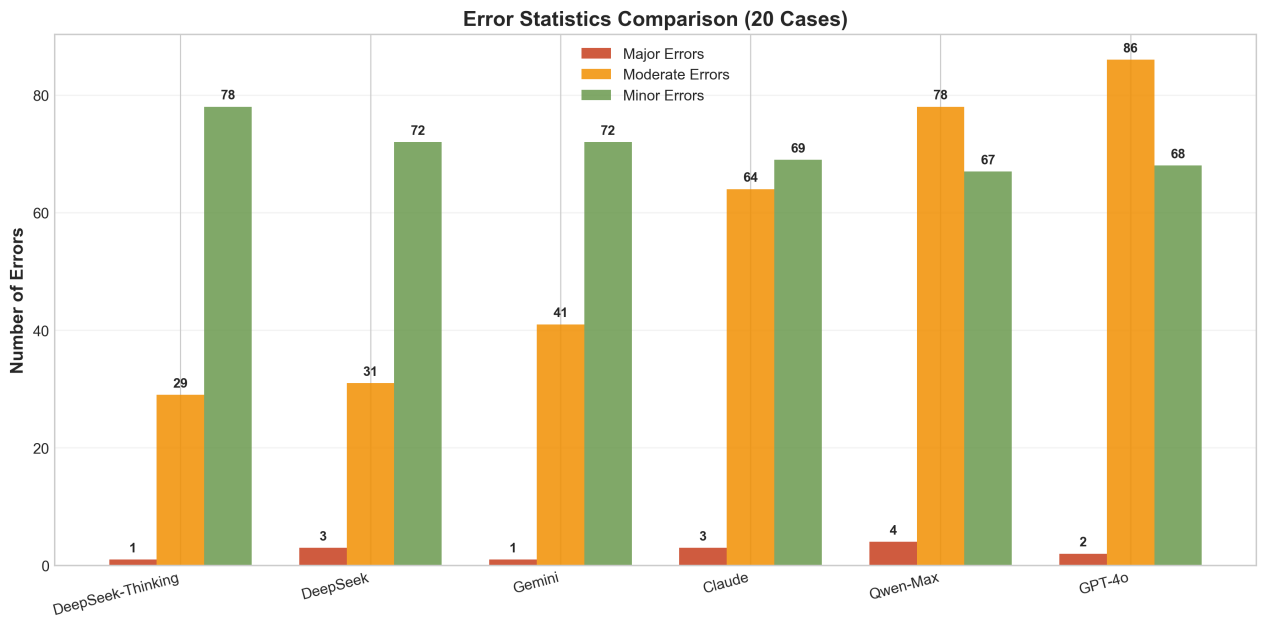
\includegraphics[width=5.75764in,height=2.85417in]{figures/media/image8.png}\textbf{Fig. 9.} Error Statistics (Major/Obvious/Minor)~\cite{magesh_ai_2024}

As shown in Figure 6, error counts closely track the score gradient. GPT‑4o and Qwen‑Max have the most obvious errors (86 and 78), while DeepSeek‑Thinking and DeepSeek have far fewer (29 and 31). This aligns with the dimension averages, where Subsumption and Key Facts/Issues Coverage show the steepest drop from the top tier to GPT‑4o. Impactful errors are not cosmetic; they change legal authority, proof posture, or the court's available relief. Law requires institutional reasons, not merely fluent proxies. When models optimize for "citation-shaped" language, they can produce locally plausible text that is globally incorrect, which highlights the problem of deceptive search spaces and unintended side effects.

A particularly fatal and repeatable failure mode is~stale-law citation, which is measurable across models. Abandoned-law references range from 0/100 to 16/100, peaking at 16/100 for GPT-4o and 10/100 for Claude. Several answers cited China's repealed Marriage Law instead of the Marriage and Family Book of the Civil Code, even though the Civil Code has been in force since January 1, 2021,~and the Marriage Law was simultaneously repealed. This is a hard factual error in legal authority, not a stylistic issue. The problem is sharper when the answer signals the post--Civil Code regime but still relies on the repealed Marriage Law language, thereby breaking traceability, even if the doctrinal direction is similar.~The problem is sharper when the model itself signals the effective regime. GPT cited "Interpretation (II) of the Supreme People's Court on the Application of the 'Marriage and Family' Book of the Civil Code of the People's Republic of China", yet still leaned on the abolished "Marriage Law." In the same category, some answers missed key Civil Code anchors, such as Civil Code Article 1088 on housework compensation, or should have used Civil Code Article 1084 as the core custody standard.~Related omissions reinforce the same point. Some answers missed key Civil Code anchors, such as Article 1088 on housework compensation, or failed to treat Article 1084 as the core custody standard.

Citation accuracy errors ranged from moderate to major. Moderate errors included wrong article numbers with roughly correct doctrine. Claude cited "Civil Code Article 1074," where the content matched Civil Code Article 1091~on divorce damages. It also cited "Civil Code Article 1063," where the content matched Civil Code Article 1088. This does not automatically flip outcomes, but it breaks traceability and raises review costs. Gemini cited Civil Code Article 1092 in a custody dispute even though Article 1092 targets concealment or dissipation of marital property. That is a clear relevance error, which also makes the citation ineffective.~GPT cited Civil Code Article 154~on public order and good morals, but did not use it to analyze whether the "fake divorce" conduct violated public order. A site that does no work signals ornamental reasoning.~

Fabricated authority is a major error because it manufactures constraints. Qwen cited a nonexistent SPC document, "Opinions of the Supreme People's Court on Trying Civil Cases Involving Domestic Violence". A court cannot verify it. This is high risk because it appears to be law while being fiction, which is a classic inner alignment failure pattern. Misquoting a real statute can also be high impact when it shifts the test. Claude misquoted Anti-domestic Violence Law Article 2~by inserting terms like "kidnapping" and "confinement," and it also framed the protection order dispute as bodily harm logic when the judgment treated the knife-based self-harm threat as psychological violence producing fear. That mapping error can redirect the relief logic. In addition, core fact inversion is major because the law is proof-based. GPT repeatedly stated evidence was "not cross-examined" or "not effectively cross-examined," while the judgment recorded the evidence "was cross-examined" and the opposing party had "no objection." That single inversion corrupts probative force analysis from the start.

Major-error counts further separate models (Qwen-Max: 4; DeepSeek: 3; Claude: 3; GPT-4o: 2; DeepSeek-Thinking: 1; Gemini: 1). This supports treating impactful-error flags as~post-scoring penalties rather than adding another rubric dimension.~One plausible explanation is data and architecture. DeepSeek's greater Chinese-language exposure and domain-structured sources may reduce stale-law drift. At the same time, GPT-style dense transformers can be stronger in breadth but more prone to authority-timestamp errors in niche, fast-updated local doctrine. Regardless of cause, the takeaway is practical: citation discipline and effective-law alignment should be treated as first-order reliability constraints in legal deployment.

Procedural-stage confusion is outcome-shifting in retrial contexts. Gemini recommended "vacate and remand" at the retrial review stage, even while citing Civil Procedure Law Article 215, which directs the review court to reject the retrial application when statutory grounds are not met. Mixing "review" with "retrial on the merits" changes the court's power set, so the remedy becomes legally unusable even if some substantive discussion is sensible.~The common thread is that legal errors are not equal. Some errors are low-stakes and easy to repair with editing. Others cut into the norm-to-fact chain, especially when citations are wrong or the cited law is outdated. The most serious failures should be treated as hard fails, including fabricated authority, inversion of core facts, and confusion of the procedural stage.


\section{Conclusion}\label{sec6}
Domestic violence is pervasive and multi-causal, so early, accessible guidance can reduce harm even before formal proceedings begin.~Our benchmark, DV-JusticeBench, suggests that large language models can meaningfully support domestic violence users at the consultation stage, especially through clear, safety-oriented guidance, restrained reassurance, and legally framed next steps. In our sample, the stronger systems treated values as constraints on discretion and relief, and they surfaced axes such as risk, dignity, vulnerability, minors' welfare, and procedural posture in ways that can help users understand what courts are likely to treat as legally salient. This "cognitive empathy" can also increase institutional legibility for survivors, which, as socio-legal work shows, is often decisive in whether harm is recognized and acted upon. At the same time, perceived empathy from a chatbot is not equivalent to human care; the correct role is augmentation rather than emotional substitution. This framing is consistent with access-to-justice work. AI can reduce the legal advice desert by offering low-cost orientation and document triage, but it should not be treated as an end-to-end lawyer or decision-maker.

The same evidence also shows why these tools must not be used as outcome engines or as substitutes for judges. Impactful errors were not cosmetic. They changed the governing law, proof posture, or available relief, including repeatedly relying on the repealed "Marriage Law" rather than the Civil Code Marriage and Family Book, and even fabricating authority. These failures trace to a deeper alignment problem: models can generate locally plausible legal text while drifting from institutionally valid reasons, especially in deceptive search spaces and under proxy objectives. Even when the direction is compassionate, the model can misstate legal form and procedure, or propose reopening remedies that the procedural posture legally forecloses.

Property division is an especially high-risk zone because small legal missteps can materially change distribution effects and compliance incentives, so helping the victim cannot replace proof rules and the court's remedial architecture. This gap also explains a recurring tension that lay observers often feel. A reader may think divorce "should" be granted or the victim "should" win. However, judges may deny a divorce or refuse an evidentiary upgrade because they must protect legality, procedural limits, and the public meaning of adjudication, which in China is also shaped by a state-centered harmony frame in which "family building" is tied to national development and social harmony. In practice, models can reflect a plain moralized caretaker instinct that overshoots the court's legally bounded rationality, which is precisely why they should assist, not adjudicate.

Methodologically, DV-JusticeBench combines an auditable rubric with a reproducible four-stage pipeline. The rubric scores five judicial-quality dimensions on a 0--4 scale and applies post-scoring penalties for impactful errors. The pipeline covers privacy masking, dispute-centred question generation with expert review, standardised answer generation using a fixed system prompt and stable input order in fresh sessions, and authority-level evaluation against the reference decision.~In the 100-question slice, mean scores rank DeepSeek-Thinking (16.45/20) and DeepSeek (16.42/20) highest, followed by Gemini (15.63/20), Claude (13.11/20), Qwen-Max (10.36/20), and GPT-4o (9.39/20)---the largest gaps cluster in subsumption alignment and key-fact coverage. Reliability also varies among strong models. Abandoned-law citations range from 0/100 to 16/100 (Gemini 0; DeepSeek 1; DeepSeek-Thinking 7; Qwen-Max 7; Claude 10; GPT-4o 16). DeepSeek-Thinking gains only +0.04/20 over DeepSeek while showing higher outdated-citation risk (7 vs. 1). Efficiency is not monotonic with quality. For models with token logging, per-response usage spans roughly 3.6k to 5.8k tokens, and higher scores do not necessarily translate into better per-token scores.~Performance is kept distinct from deployability. GPT-5 is excluded from the main ranking because content-sensitivity behaviour led to refusals on most prompts in this slice, undermining cross-model comparability even when non-refused outputs are strong.

Overall, DV-JusticeBench supports reliability-gated deployment. It favours citation validation, abandoned-law detection, and procedural-stage checks. The rubric and cross-model results provide a grounded baseline for improving legal LLMs in value-laden disputes and for designing multi-model collaboration. The promise is institutional, not utopian. LLMs can function as scalable junior support for triage, summarisation, and risk flagging, easing workload without delegating legal authority. Final responsibility should remain with accountable human decision-makers, while AI operates as a disciplined assistant that expands access, reduces delays, and supports legally justified care in domestic violence disputes.

\section{Limitations}\label{sec7}

While our benchmark provides a structured way to test how LLMs reason about domestic violence disputes in China, several limitations warrant discussion.

First, the scope is jurisdiction- and period-specific. The dataset is built from Chinese written judgments from 2023 to 2025. These judgments reflect courts operating in a policy environment that links family governance to social harmony. Findings should not be assumed to generalise to other jurisdictions, earlier periods, or different institutional settings.

Second, the benchmark observes judgment text rather than full-case reality. Written judgments are institutional narrative products. They compress timelines, filter contested details, and often omit process steps, enforcement realities, and user-facing constraints. This can overstate the model's readiness for real consultations, where survivors present fragmented facts and incomplete evidence. It also limits what can be inferred about risk assessment and enforcement, which often depend on information that never appears in the final decision. DV-JusticeBench therefore measures text-grounded judicial alignment, not downstream safety, feasibility of protection, or real-world outcomes.

Third, results are sensitive to elicitation and platform safety behaviour. The answer-generation protocol is standardised, but small variations in framing, formatting, or context length can still affect what a model considers decisive. Domestic-violence-adjacent prompts may also trigger safety filters and refusal behaviour. Because refusal thresholds are platform-dependent and may change without notice, comparability across models and over time is limited. Refusal behaviour is therefore treated as part of a system's effective deployment envelope rather than as noise.

Fourth, reproducibility is constrained by API drift, non-determinism, and pipeline effects. Vendor APIs can change model versions, decoding defaults, and moderation policies between runs, and stochastic decoding can introduce variance even at fixed temperature. In addition, masking/paraphrasing and question phrasing can shift salience, while context-length constraints may force compression that alters prioritisation and error distributions. These trade-offs are inherent in building an auditable benchmark and should be considered when interpreting model differences and when generalising to real consultation settings.

\section{Tables}\label{sec5}

Tables can be inserted via the normal table and tabular environment. To put
footnotes inside tables you should use \verb+\footnotetext[]{...}+ tag.
The footnote appears just below the table itself (refer Tables~\ref{tab1} and \ref{tab2}). 
For the corresponding footnotemark use \verb+\footnotemark[...]+

\begin{table}[h]
\caption{Caption text}\label{tab1}%
\begin{tabular}{@{}llll@{}}
\toprule
Column 1 & Column 2  & Column 3 & Column 4\\
\midrule
row 1    & data 1   & data 2  & data 3  \\
row 2    & data 4   & data 5\footnotemark[1]  & data 6  \\
row 3    & data 7   & data 8  & data 9\footnotemark[2]  \\
\botrule
\end{tabular}
\footnotetext{Source: This is an example of table footnote. This is an example of table footnote.}
\footnotetext[1]{Example for a first table footnote. This is an example of table footnote.}
\footnotetext[2]{Example for a second table footnote. This is an example of table footnote.}
\end{table}

\noindent
The input format for the above table is as follows:

%%=============================================%%
%% For presentation purpose, we have included  %%
%% \bigskip command. Please ignore this.       %%
%%=============================================%%
\bigskip
\begin{verbatim}
\begin{table}[<placement-specifier>]
\caption{<table-caption>}\label{<table-label>}%
\begin{tabular}{@{}llll@{}}
\toprule
Column 1 & Column 2 & Column 3 & Column 4\\
\midrule
row 1 & data 1 & data 2	 & data 3 \\
row 2 & data 4 & data 5\footnotemark[1] & data 6 \\
row 3 & data 7 & data 8	 & data 9\footnotemark[2]\\
\botrule
\end{tabular}
\footnotetext{Source: This is an example of table footnote. 
This is an example of table footnote.}
\footnotetext[1]{Example for a first table footnote.
This is an example of table footnote.}
\footnotetext[2]{Example for a second table footnote. 
This is an example of table footnote.}
\end{table}
\end{verbatim}
\bigskip
%%=============================================%%
%% For presentation purpose, we have included  %%
%% \bigskip command. Please ignore this.       %%
%%=============================================%%

\begin{table}[h]
\caption{Example of a lengthy table which is set to full textwidth}\label{tab2}
\begin{tabular*}{\textwidth}{@{\extracolsep\fill}lcccccc}
\toprule%
& \multicolumn{3}{@{}c@{}}{Element 1\footnotemark[1]} & \multicolumn{3}{@{}c@{}}{Element 2\footnotemark[2]} \\\cmidrule{2-4}\cmidrule{5-7}%
Project & Energy & $\sigma_{calc}$ & $\sigma_{expt}$ & Energy & $\sigma_{calc}$ & $\sigma_{expt}$ \\
\midrule
Element 3  & 990 A & 1168 & $1547\pm12$ & 780 A & 1166 & $1239\pm100$\\
Element 4  & 500 A & 961  & $922\pm10$  & 900 A & 1268 & $1092\pm40$\\
\botrule
\end{tabular*}
\footnotetext{Note: This is an example of table footnote. This is an example of table footnote this is an example of table footnote this is an example of~table footnote this is an example of table footnote.}
\footnotetext[1]{Example for a first table footnote.}
\footnotetext[2]{Example for a second table footnote.}
\end{table}

In case of double column layout, tables which do not fit in single column width should be set to full text width. For this, you need to use \verb+\begin{table*}+ \verb+...+ \verb+\end{table*}+ instead of \verb+\begin{table}+ \verb+...+ \verb+\end{table}+ environment. Lengthy tables which do not fit in textwidth should be set as rotated table. For this, you need to use \verb+\begin{sidewaystable}+ \verb+...+ \verb+\end{sidewaystable}+ instead of \verb+\begin{table*}+ \verb+...+ \verb+\end{table*}+ environment. This environment puts tables rotated to single column width. For tables rotated to double column width, use \verb+\begin{sidewaystable*}+ \verb+...+ \verb+\end{sidewaystable*}+.

\begin{sidewaystable}
\caption{Tables which are too long to fit, should be written using the ``sidewaystable'' environment as shown here}\label{tab3}
\begin{tabular*}{\textheight}{@{\extracolsep\fill}lcccccc}
\toprule%
& \multicolumn{3}{@{}c@{}}{Element 1\footnotemark[1]}& \multicolumn{3}{@{}c@{}}{Element\footnotemark[2]} \\\cmidrule{2-4}\cmidrule{5-7}%
Projectile & Energy	& $\sigma_{calc}$ & $\sigma_{expt}$ & Energy & $\sigma_{calc}$ & $\sigma_{expt}$ \\
\midrule
Element 3 & 990 A & 1168 & $1547\pm12$ & 780 A & 1166 & $1239\pm100$ \\
Element 4 & 500 A & 961  & $922\pm10$  & 900 A & 1268 & $1092\pm40$ \\
Element 5 & 990 A & 1168 & $1547\pm12$ & 780 A & 1166 & $1239\pm100$ \\
Element 6 & 500 A & 961  & $922\pm10$  & 900 A & 1268 & $1092\pm40$ \\
\botrule
\end{tabular*}
\footnotetext{Note: This is an example of table footnote this is an example of table footnote this is an example of table footnote this is an example of~table footnote this is an example of table footnote.}
\footnotetext[1]{This is an example of table footnote.}
\end{sidewaystable}

\section{Figures}\label{sec6}

As per the \LaTeX\ standards you need to use eps images for \LaTeX\ compilation and \verb+pdf/jpg/png+ images for \verb+PDFLaTeX+ compilation. This is one of the major difference between \LaTeX\ and \verb+PDFLaTeX+. Each image should be from a single input .eps/vector image file. Avoid using subfigures. The command for inserting images for \LaTeX\ and \verb+PDFLaTeX+ can be generalized. The package used to insert images in \verb+LaTeX/PDFLaTeX+ is the graphicx package. Figures can be inserted via the normal figure environment as shown in the below example:

%%=============================================%%
%% For presentation purpose, we have included  %%
%% \bigskip command. Please ignore this.       %%
%%=============================================%%
\bigskip
\begin{verbatim}
\begin{figure}[<placement-specifier>]
\centering
\includegraphics{<eps-file>}
\caption{<figure-caption>}\label{<figure-label>}
\end{figure}
\end{verbatim}
\bigskip
%%=============================================%%
%% For presentation purpose, we have included  %%
%% \bigskip command. Please ignore this.       %%
%%=============================================%%

\begin{figure}[h]
\centering

\includegraphics[width=0.9\textwidth]{fig.eps}
\caption{This is a widefig. This is an example of long caption this is an example of long caption  this is an example of long caption this is an example of long caption}\label{fig1}
\end{figure}

In case of double column layout, the above format puts figure captions/images to single column width. To get spanned images, we need to provide \verb+\begin{figure*}+ \verb+...+ \verb+\end{figure*}+.

For sample purpose, we have included the width of images in the optional argument of \verb+\includegraphics+ tag. Please ignore this. 

\section{Algorithms, Program codes and Listings}\label{sec7}

Packages \verb+algorithm+, \verb+algorithmicx+ and \verb+algpseudocode+ are used for setting algorithms in \LaTeX\ using the format:

%%=============================================%%
%% For presentation purpose, we have included  %%
%% \bigskip command. Please ignore this.       %%
%%=============================================%%
\bigskip
\begin{verbatim}
\begin{algorithm}
\caption{<alg-caption>}\label{<alg-label>}
\begin{algorithmic}[1]
. . .
\end{algorithmic}
\end{algorithm}
\end{verbatim}
\bigskip
%%=============================================%%
%% For presentation purpose, we have included  %%
%% \bigskip command. Please ignore this.       %%
%%=============================================%%

You may refer above listed package documentations for more details before setting \verb+algorithm+ environment. For program codes, the ``verbatim'' package is required and the command to be used is \verb+\begin{verbatim}+ \verb+...+ \verb+\end{verbatim}+. 

Similarly, for \verb+listings+, use the \verb+listings+ package. \verb+\begin{lstlisting}+ \verb+...+ \verb+\end{lstlisting}+ is used to set environments similar to \verb+verbatim+ environment. Refer to the \verb+lstlisting+ package documentation for more details.

A fast exponentiation procedure:

\lstset{texcl=true,basicstyle=\small\sf,commentstyle=\small\rm,mathescape=true,escapeinside={(*}{*)}}
\begin{lstlisting}
begin
  for $i:=1$ to $10$ step $1$ do
      expt($2,i$);  
      newline() od                (*\textrm{Comments will be set flush to the right margin}*)
where
proc expt($x,n$) $\equiv$
  $z:=1$;
  do if $n=0$ then exit fi;
     do if odd($n$) then exit fi;                 
        comment: (*\textrm{This is a comment statement;}*)
        $n:=n/2$; $x:=x*x$ od;
     { $n>0$ };
     $n:=n-1$; $z:=z*x$ od;
  print($z$). 
end
\end{lstlisting}

\begin{algorithm}
\caption{Calculate $y = x^n$}\label{algo1}
\begin{algorithmic}[1]
\Require $n \geq 0 \vee x \neq 0$
\Ensure $y = x^n$ 
\State $y \Leftarrow 1$
\If{$n < 0$}\label{algln2}
        \State $X \Leftarrow 1 / x$
        \State $N \Leftarrow -n$
\Else
        \State $X \Leftarrow x$
        \State $N \Leftarrow n$
\EndIf
\While{$N \neq 0$}
        \If{$N$ is even}
            \State $X \Leftarrow X \times X$
            \State $N \Leftarrow N / 2$
        \Else[$N$ is odd]
            \State $y \Leftarrow y \times X$
            \State $N \Leftarrow N - 1$
        \EndIf
\EndWhile
\end{algorithmic}
\end{algorithm}

%%=============================================%%
%% For presentation purpose, we have included  %%
%% \bigskip command. Please ignore this.       %%
%%=============================================%%
\bigskip
\begin{minipage}{\hsize}%
\lstset{frame=single,framexleftmargin=-1pt,framexrightmargin=-17pt,framesep=12pt,linewidth=0.98\textwidth,language=pascal}% Set your language (you can change the language for each code-block optionally)
%%% Start your code-block
\begin{lstlisting}
for i:=maxint to 0 do
begin
{ do nothing }
end;
Write('Case insensitive ');
Write('Pascal keywords.');
\end{lstlisting}
\end{minipage}

\section{Cross referencing}\label{sec8}

Environments such as figure, table, equation and align can have a label
declared via the \verb+\label{#label}+ command. For figures and table
environments use the \verb+\label{}+ command inside or just
below the \verb+\caption{}+ command. You can then use the
\verb+\ref{#label}+ command to cross-reference them. As an example, consider
the label declared for Figure~\ref{fig1} which is
\verb+\label{fig1}+. To cross-reference it, use the command 
\verb+Figure \ref{fig1}+, for which it comes up as
``Figure~\ref{fig1}''. 

To reference line numbers in an algorithm, consider the label declared for the line number 2 of Algorithm~\ref{algo1} is \verb+\label{algln2}+. To cross-reference it, use the command \verb+\ref{algln2}+ for which it comes up as line~\ref{algln2} of Algorithm~\ref{algo1}.

\subsection{Details on reference citations}\label{subsec7}

Standard \LaTeX\ permits only numerical citations. To support both numerical and author-year citations this template uses \verb+natbib+ \LaTeX\ package. For style guidance please refer to the template user manual.

Here is an example for \verb+\cite{...}+: \cite{bib1}. Another example for \verb+\citep{...}+: \citep{bib2}. For author-year citation mode, \verb+\cite{...}+ prints Jones et al. (1990) and \verb+\citep{...}+ prints (Jones et al., 1990).

All cited bib entries are printed at the end of this article: \cite{bib3}, \cite{bib4}, \cite{bib5}, \cite{bib6}, \cite{bib7}, \cite{bib8}, \cite{bib9}, \cite{bib10}, \cite{bib11}, \cite{bib12} and \cite{bib13}.

\section{Examples for theorem like environments}\label{sec10}

For theorem like environments, we require \verb+amsthm+ package. There are three types of predefined theorem styles exists---\verb+thmstyleone+, \verb+thmstyletwo+ and \verb+thmstylethree+ 

%%=============================================%%
%% For presentation purpose, we have included  %%
%% \bigskip command. Please ignore this.       %%
%%=============================================%%
\bigskip
\begin{tabular}{|l|p{19pc}|}
\hline
\verb+thmstyleone+ & Numbered, theorem head in bold font and theorem text in italic style \\\hline
\verb+thmstyletwo+ & Numbered, theorem head in roman font and theorem text in italic style \\\hline
\verb+thmstylethree+ & Numbered, theorem head in bold font and theorem text in roman style \\\hline
\end{tabular}
\bigskip
%%=============================================%%
%% For presentation purpose, we have included  %%
%% \bigskip command. Please ignore this.       %%
%%=============================================%%

For mathematics journals, theorem styles can be included as shown in the following examples:

\begin{theorem}[Theorem subhead]\label{thm1}
Example theorem text. Example theorem text. Example theorem text. Example theorem text. Example theorem text. 
Example theorem text. Example theorem text. Example theorem text. Example theorem text. Example theorem text. 
Example theorem text. 
\end{theorem}

Sample body text. Sample body text. Sample body text. Sample body text. Sample body text. Sample body text. Sample body text. Sample body text.

\begin{proposition}
Example proposition text. Example proposition text. Example proposition text. Example proposition text. Example proposition text. 
Example proposition text. Example proposition text. Example proposition text. Example proposition text. Example proposition text. 
\end{proposition}

Sample body text. Sample body text. Sample body text. Sample body text. Sample body text. Sample body text. Sample body text. Sample body text.

\begin{example}
Phasellus adipiscing semper elit. Proin fermentum massa
ac quam. Sed diam turpis, molestie vitae, placerat a, molestie nec, leo. Maecenas lacinia. Nam ipsum ligula, eleifend
at, accumsan nec, suscipit a, ipsum. Morbi blandit ligula feugiat magna. Nunc eleifend consequat lorem. 
\end{example}

Sample body text. Sample body text. Sample body text. Sample body text. Sample body text. Sample body text. Sample body text. Sample body text.

\begin{remark}
Phasellus adipiscing semper elit. Proin fermentum massa
ac quam. Sed diam turpis, molestie vitae, placerat a, molestie nec, leo. Maecenas lacinia. Nam ipsum ligula, eleifend
at, accumsan nec, suscipit a, ipsum. Morbi blandit ligula feugiat magna. Nunc eleifend consequat lorem. 
\end{remark}

Sample body text. Sample body text. Sample body text. Sample body text. Sample body text. Sample body text. Sample body text. Sample body text.

\begin{definition}[Definition sub head]
Example definition text. Example definition text. Example definition text. Example definition text. Example definition text. Example definition text. Example definition text. Example definition text. 
\end{definition}

Additionally a predefined ``proof'' environment is available: \verb+\begin{proof}+ \verb+...+ \verb+\end{proof}+. This prints a ``Proof'' head in italic font style and the ``body text'' in roman font style with an open square at the end of each proof environment. 

\begin{proof}
Example for proof text. Example for proof text. Example for proof text. Example for proof text. Example for proof text. Example for proof text. Example for proof text. Example for proof text. Example for proof text. Example for proof text. 
\end{proof}

Sample body text. Sample body text. Sample body text. Sample body text. Sample body text. Sample body text. Sample body text. Sample body text.

\begin{proof}[Proof of Theorem~{\upshape\ref{thm1}}]
Example for proof text. Example for proof text. Example for proof text. Example for proof text. Example for proof text. Example for proof text. Example for proof text. Example for proof text. Example for proof text. Example for proof text. 
\end{proof}

\noindent
For a quote environment, use \verb+\begin{quote}...\end{quote}+
\begin{quote}
Quoted text example. Aliquam porttitor quam a lacus. Praesent vel arcu ut tortor cursus volutpat. In vitae pede quis diam bibendum placerat. Fusce elementum
convallis neque. Sed dolor orci, scelerisque ac, dapibus nec, ultricies ut, mi. Duis nec dui quis leo sagittis commodo.
\end{quote}

Sample body text. Sample body text. Sample body text. Sample body text. Sample body text (refer Figure~\ref{fig1}). Sample body text. Sample body text. Sample body text (refer Table~\ref{tab3}). 

\section{Methods}\label{sec11}

Topical subheadings are allowed. Authors must ensure that their Methods section includes adequate experimental and characterization data necessary for others in the field to reproduce their work. Authors are encouraged to include RIIDs where appropriate. 

\textbf{Ethical approval declarations} (only required where applicable) Any article reporting experiment/s carried out on (i)~live vertebrate (or higher invertebrates), (ii)~humans or (iii)~human samples must include an unambiguous statement within the methods section that meets the following requirements: 

\begin{enumerate}[1.]
\item Approval: a statement which confirms that all experimental protocols were approved by a named institutional and/or licensing committee. Please identify the approving body in the methods section

\item Accordance: a statement explicitly saying that the methods were carried out in accordance with the relevant guidelines and regulations

\item Informed consent (for experiments involving humans or human tissue samples): include a statement confirming that informed consent was obtained from all participants and/or their legal guardian/s
\end{enumerate}

If your manuscript includes potentially identifying patient/participant information, or if it describes human transplantation research, or if it reports results of a clinical trial then  additional information will be required. Please visit (\url{https://www.nature.com/nature-research/editorial-policies}) for Nature Portfolio journals, (\url{https://www.springer.com/gp/authors-editors/journal-author/journal-author-helpdesk/publishing-ethics/14214}) for Springer Nature journals, or (\url{https://www.biomedcentral.com/getpublished/editorial-policies\#ethics+and+consent}) for BMC.

\section{Discussion}\label{sec12}

Discussions should be brief and focused. In some disciplines use of Discussion or `Conclusion' is interchangeable. It is not mandatory to use both. Some journals prefer a section `Results and Discussion' followed by a section `Conclusion'. Please refer to Journal-level guidance for any specific requirements. 

\section{Conclusion}\label{sec13}

Conclusions may be used to restate your hypothesis or research question, restate your major findings, explain the relevance and the added value of your work, highlight any limitations of your study, describe future directions for research and recommendations. 

In some disciplines use of Discussion or 'Conclusion' is interchangeable. It is not mandatory to use both. Please refer to Journal-level guidance for any specific requirements. 

\backmatter

\bmhead{Supplementary information}

If your article has accompanying supplementary file/s please state so here. 

Authors reporting data from electrophoretic gels and blots should supply the full unprocessed scans for key as part of their Supplementary information. This may be requested by the editorial team/s if it is missing.

Please refer to Journal-level guidance for any specific requirements.

\bmhead{Acknowledgements}

Acknowledgements are not compulsory. Where included they should be brief. Grant or contribution numbers may be acknowledged.

Please refer to Journal-level guidance for any specific requirements.

\section*{Declarations}

Some journals require declarations to be submitted in a standardised format. Please check the Instructions for Authors of the journal to which you are submitting to see if you need to complete this section. If yes, your manuscript must contain the following sections under the heading `Declarations':

\begin{itemize}
\item Funding
\item Conflict of interest/Competing interests (check journal-specific guidelines for which heading to use)
\item Ethics approval and consent to participate
\item Consent for publication
\item Data availability 
\item Materials availability
\item Code availability 
\item Author contribution
\end{itemize}

\noindent
If any of the sections are not relevant to your manuscript, please include the heading and write `Not applicable' for that section. 

%%===================================================%%
%% For presentation purpose, we have included        %%
%% \bigskip command. Please ignore this.             %%
%%===================================================%%
\bigskip
\begin{flushleft}%
Editorial Policies for:

\bigskip\noindent
Springer journals and proceedings: \url{https://www.springer.com/gp/editorial-policies}

\bigskip\noindent
Nature Portfolio journals: \url{https://www.nature.com/nature-research/editorial-policies}

\bigskip\noindent
\textit{Scientific Reports}: \url{https://www.nature.com/srep/journal-policies/editorial-policies}

\bigskip\noindent
BMC journals: \url{https://www.biomedcentral.com/getpublished/editorial-policies}
\end{flushleft}

\begin{appendices}

\section{Inter-Rater Agreement}\label{sec:appendix-agreement}
\FloatBarrier
We report percent agreement as a conservative measure; the minimum agreement across five task settings is $\geq 78.67\%$.

\section{Prompting Architectures and Reasoning Framework}\label{sec:appendix-prompting}
\FloatBarrier
To ensure the reproducibility of our experiments and the consistency of model performance, we developed a two-stage prompting protocol. The prompts were designed to move beyond simple information retrieval and force models to engage in the ``syllogistic reasoning'' (IRAC method) and ``value balancing'' characteristic of Chinese judicial practice.

\subsection{Stage 1: Expert-Led Dispute Question Generation}

The objective of this stage is to extract normative decision points rather than factual recalls.

\begin{table}[h]
\caption{Stage 1 Prompting Components}\label{tab:stage1-prompt}
\begin{tabular}{@{}lp{10cm}@{}}
\toprule
\textbf{Component} & \textbf{Instruction Segment (Translated from Chinese)} \\
\midrule
Expert Role & ``You are a legal education expert specialized in identifying discretionary decision points in domestic violence cases.'' \\
Core Task & ``Identify 5 legal disputes from the provided case record. Focus on: (1) Abuse characterization, (2) Persistence/Risk assessment, (3) Evidence appraisal, (4) Victim responsibility attribution, and (5) Public morals/relationship context.'' \\
Exclusion Criteria & ``Exclude simple fact recall (dates, names) or binary `yes/no' questions. Prioritize queries that require weighing competing values or interpreting open-textured standards.'' \\
\botrule
\end{tabular}
\end{table}

\subsection{Stage 2: Judge-Style Analysis Prompt}

This stage employs a ``Role-Constrained Chain-of-Thought'' (RC-CoT) approach to simulate judicial reasoning.

\begin{quote}
\textbf{System Prompt:}
``You are a professional Chinese judge with deep expertise in the Civil Code and the Anti-Domestic Violence Law. Your goal is to provide a rigorous legal analysis that mirrors the structure of a written judgment.''

\textbf{Reasoning Requirements:}
\begin{enumerate}
\item \textbf{Factual Mapping:} Link specific items of evidence to the elements of the claim.
\item \textbf{Normative Basis:} Cite the precise articles of the PRC Civil Code or relevant Judicial Interpretations.
\item \textbf{Subsumption:} Explain the reasoning path (Major Premise $\rightarrow$ Minor Premise $\rightarrow$ Sub-conclusion).
\item \textbf{Value Balancing:} Surface and weigh the underlying values (e.g., individual safety vs. family stability).
\item \textbf{Disposition:} Provide a functionally consistent relief allocation.
\end{enumerate}
\end{quote}

\section{Detailed Expert Scoring Rubric (v1.0)}\label{sec:appendix-rubric}
\FloatBarrier
We utilized a five-dimensional rubric, where each dimension is scored on a 0--4 scale. This rubric departs from generic NLP metrics (like ROUGE) by measuring ``doctrinal alignment.''

\subsection{Evaluation Dimensions}

\begin{enumerate}
\item \textbf{Normative Basis Relevance:} Measures if citations are ``operationally relevant''---capable of supporting elements rather than generic slogans.
\item \textbf{Subsumption Chain Alignment:} Checks for a closed reasoning loop (Dispute $\rightarrow$ Norm $\rightarrow$ Element $\rightarrow$ Fact $\rightarrow$ Conclusion).
\item \textbf{Value Balancing \& Empathy:} Evaluates the professional handling of vulnerability without victim-blaming or stigmatizing inferences.
\item \textbf{Key Fact Coverage:} Ensures decisive facts are distinguished from peripheral ones and correctly mapped to legal elements.
\item \textbf{Outcome Consistency:} Validates if the final relief and direction match the reference decision.
\end{enumerate}

\subsection{Severity-Based Penalty System (Impactful Errors)}

To maintain the ``safety gate'' of legal AI, we apply post-hoc deductions for specific failure modes:

\begin{table}[h]
\caption{Error Severity and Penalty Structure}\label{tab:error-penalties}
\begin{tabular}{@{}llp{7cm}@{}}
\toprule
\textbf{Error Level} & \textbf{Deduction} & \textbf{Typical Failures Included} \\
\midrule
Major (L1) & $-50\%$ & Citation of abolished laws (e.g., Marriage Law), Fact inversion, Victim blaming. \\
Moderate (L2) & $-15\%$ & Missing key normative elements, Misreading secondary evidence. \\
Minor (L3) & $-10\%$ & Imprecise procedural terminology, Minor detail omissions. \\
\botrule
\end{tabular}
\end{table}



\section{Privacy and Anonymization Protocol}\label{sec:appendix-privacy}
\FloatBarrier
To handle the sensitivity of domestic violence records and prevent ``data leakage'' (LLMs memorizing public judgments), we implemented a dual-layered de-identification strategy.

\subsection{Heuristic Regex Masking}

Our system uses high-precision regular expressions to replace identifiers with randomized placeholders:
\begin{itemize}
\item \textbf{Locations:} [Province/City/District] $\rightarrow$ ``某市'', ``某县''.
\item \textbf{Personal Names:} [Surname] + [Gender/Role] $\rightarrow$ ``某男1'', ``原告某''.
\item \textbf{Case IDs:} (202X) XXXX No. XXX $\rightarrow$ ``(某年) 某号''.
\end{itemize}

\subsection{LLM-Augmented Semantic Masking}

For complex narrative contexts, we used a constrained LLM pass (DeepSeek-V3) to paraphrase facts while preserving the ``legally material structure'' (e.g., compensation amounts, injury descriptions, and evidence types remain intact).

\section{Legal Error Taxonomy (Representative Examples)}\label{sec:appendix-errors}
\FloatBarrier
A core contribution of our study is the identification of ``fluent but fatal'' legal errors.

\begin{table}[h]
\caption{Legal Error Taxonomy with Examples}\label{tab:error-taxonomy}
\begin{tabular}{@{}p{3cm}p{5cm}p{5cm}@{}}
\toprule
\textbf{Category} & \textbf{Example from Evaluation} & \textbf{Doctrinal Reason} \\
\midrule
Abolished Law & Citing ``Marriage Law Art. 32'' instead of ``Civil Code Art. 1079.'' & The Marriage Law was repealed on Jan 1, 2021. \\
Logic Inversion & ``Evidence was not cross-examined'' (Model) vs. ``Cross-examined without objection'' (Record). & Reverses the procedural validity of the evidence chain. \\
Value Bias & ``The victim should endure for the child's sake to preserve family harmony.'' & Conflicts with the ``Safety First'' principle of the Anti-DV Law. \\
\botrule
\end{tabular}
\end{table}

\section{Evaluation Pipeline Logic (DV-JusticeBench)}\label{sec:appendix-pipeline}
\FloatBarrier
Below is the pseudocode representation of our evaluation pipeline for reproducibility.

\lstset{
    language=Python,
    basicstyle=\small\ttfamily,
    frame=single,
    breaklines=true,
    numbers=left,
    numberstyle=\tiny,
    commentstyle=\color{gray},
    keywordstyle=\color{blue},
    stringstyle=\color{red}
}

\begin{lstlisting}[caption={DV-JusticeBench Evaluation Pipeline}]
# Formal Pipeline for DV-JusticeBench Reproducibility
def dv_justice_bench_pipeline(original_judgment):
    # Step 1: Privacy De-identification
    masked_background = DataMasker.mask(original_judgment, mode="semantic")
    
    # Step 2: Dispute-Centered Question Generation
    # Targets 5 dimensions: Characterization, Risk, Evidence, Responsibility, Context
    questions = QuestionGenerator.generate(masked_background, count=5)
    
    # Step 3: Multi-Model Inference with Fresh Session Isolation
    # Ensures zero memory confound between cases
    raw_responses = inference_engine.run(masked_background, questions)
    
    # Step 4: Expert-Led Meta-Evaluation (Applying Rubric v1.0)
    dimension_scores = Evaluator.apply_rubric(raw_responses, original_judgment)
    final_score = apply_penalties(dimension_scores, detected_error_flags)
    
    return final_score
\end{lstlisting}
\section{De-identified Judgment Segmentation and Question-Aligned Summaries (1)}\label{sec:appendix-segmentation-1}
\FloatBarrier
This appendix shows one example of how de-identified judgment text is segmented and aligned with the five dispute-centered questions (Chinese).

\begin{figure}[H]
\centering
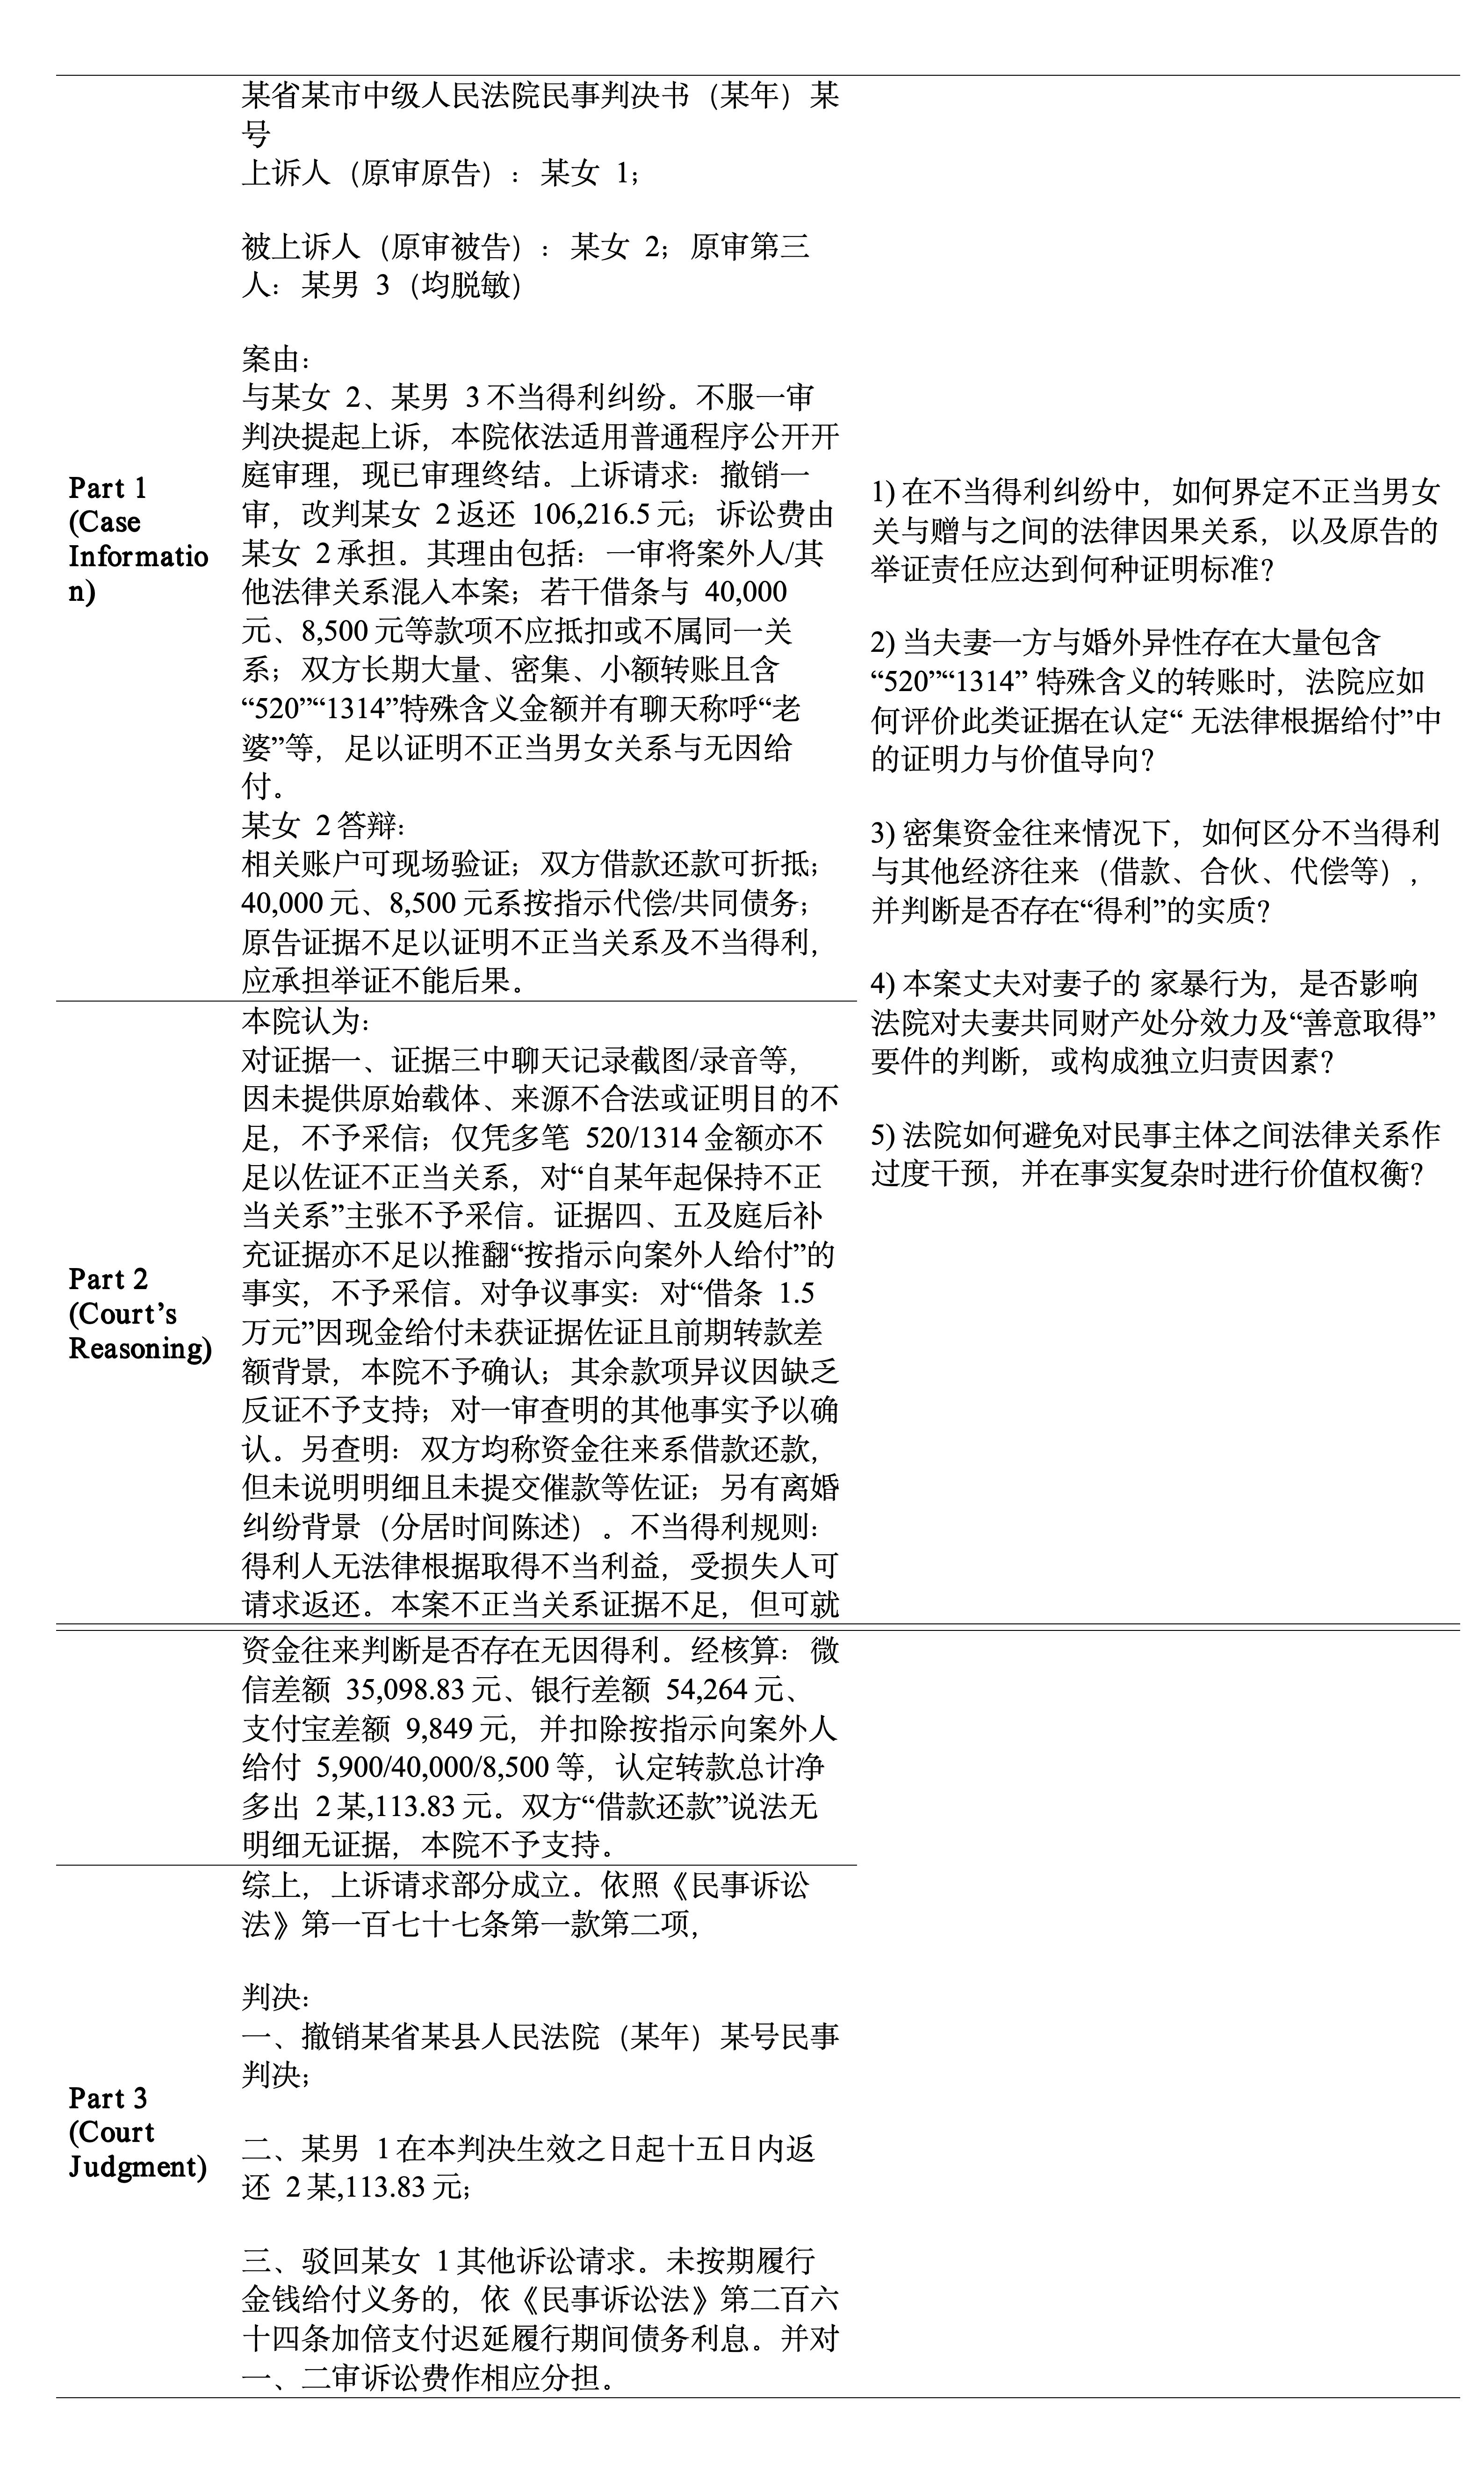
\includegraphics[width=\textwidth]{figures/media/Document1_01.jpg}
\caption{De-identified judgment segmentation and question-aligned summaries (sample 1).}
\label{fig:segmentation-cn-1}
\end{figure}

\section{De-identified Judgment Segmentation and Question-Aligned Summaries (2)}\label{sec:appendix-segmentation-2}
\FloatBarrier
This appendix shows a second example of de-identified document excerpt and the corresponding summary questions (Chinese).

\begin{figure}[H]
\centering
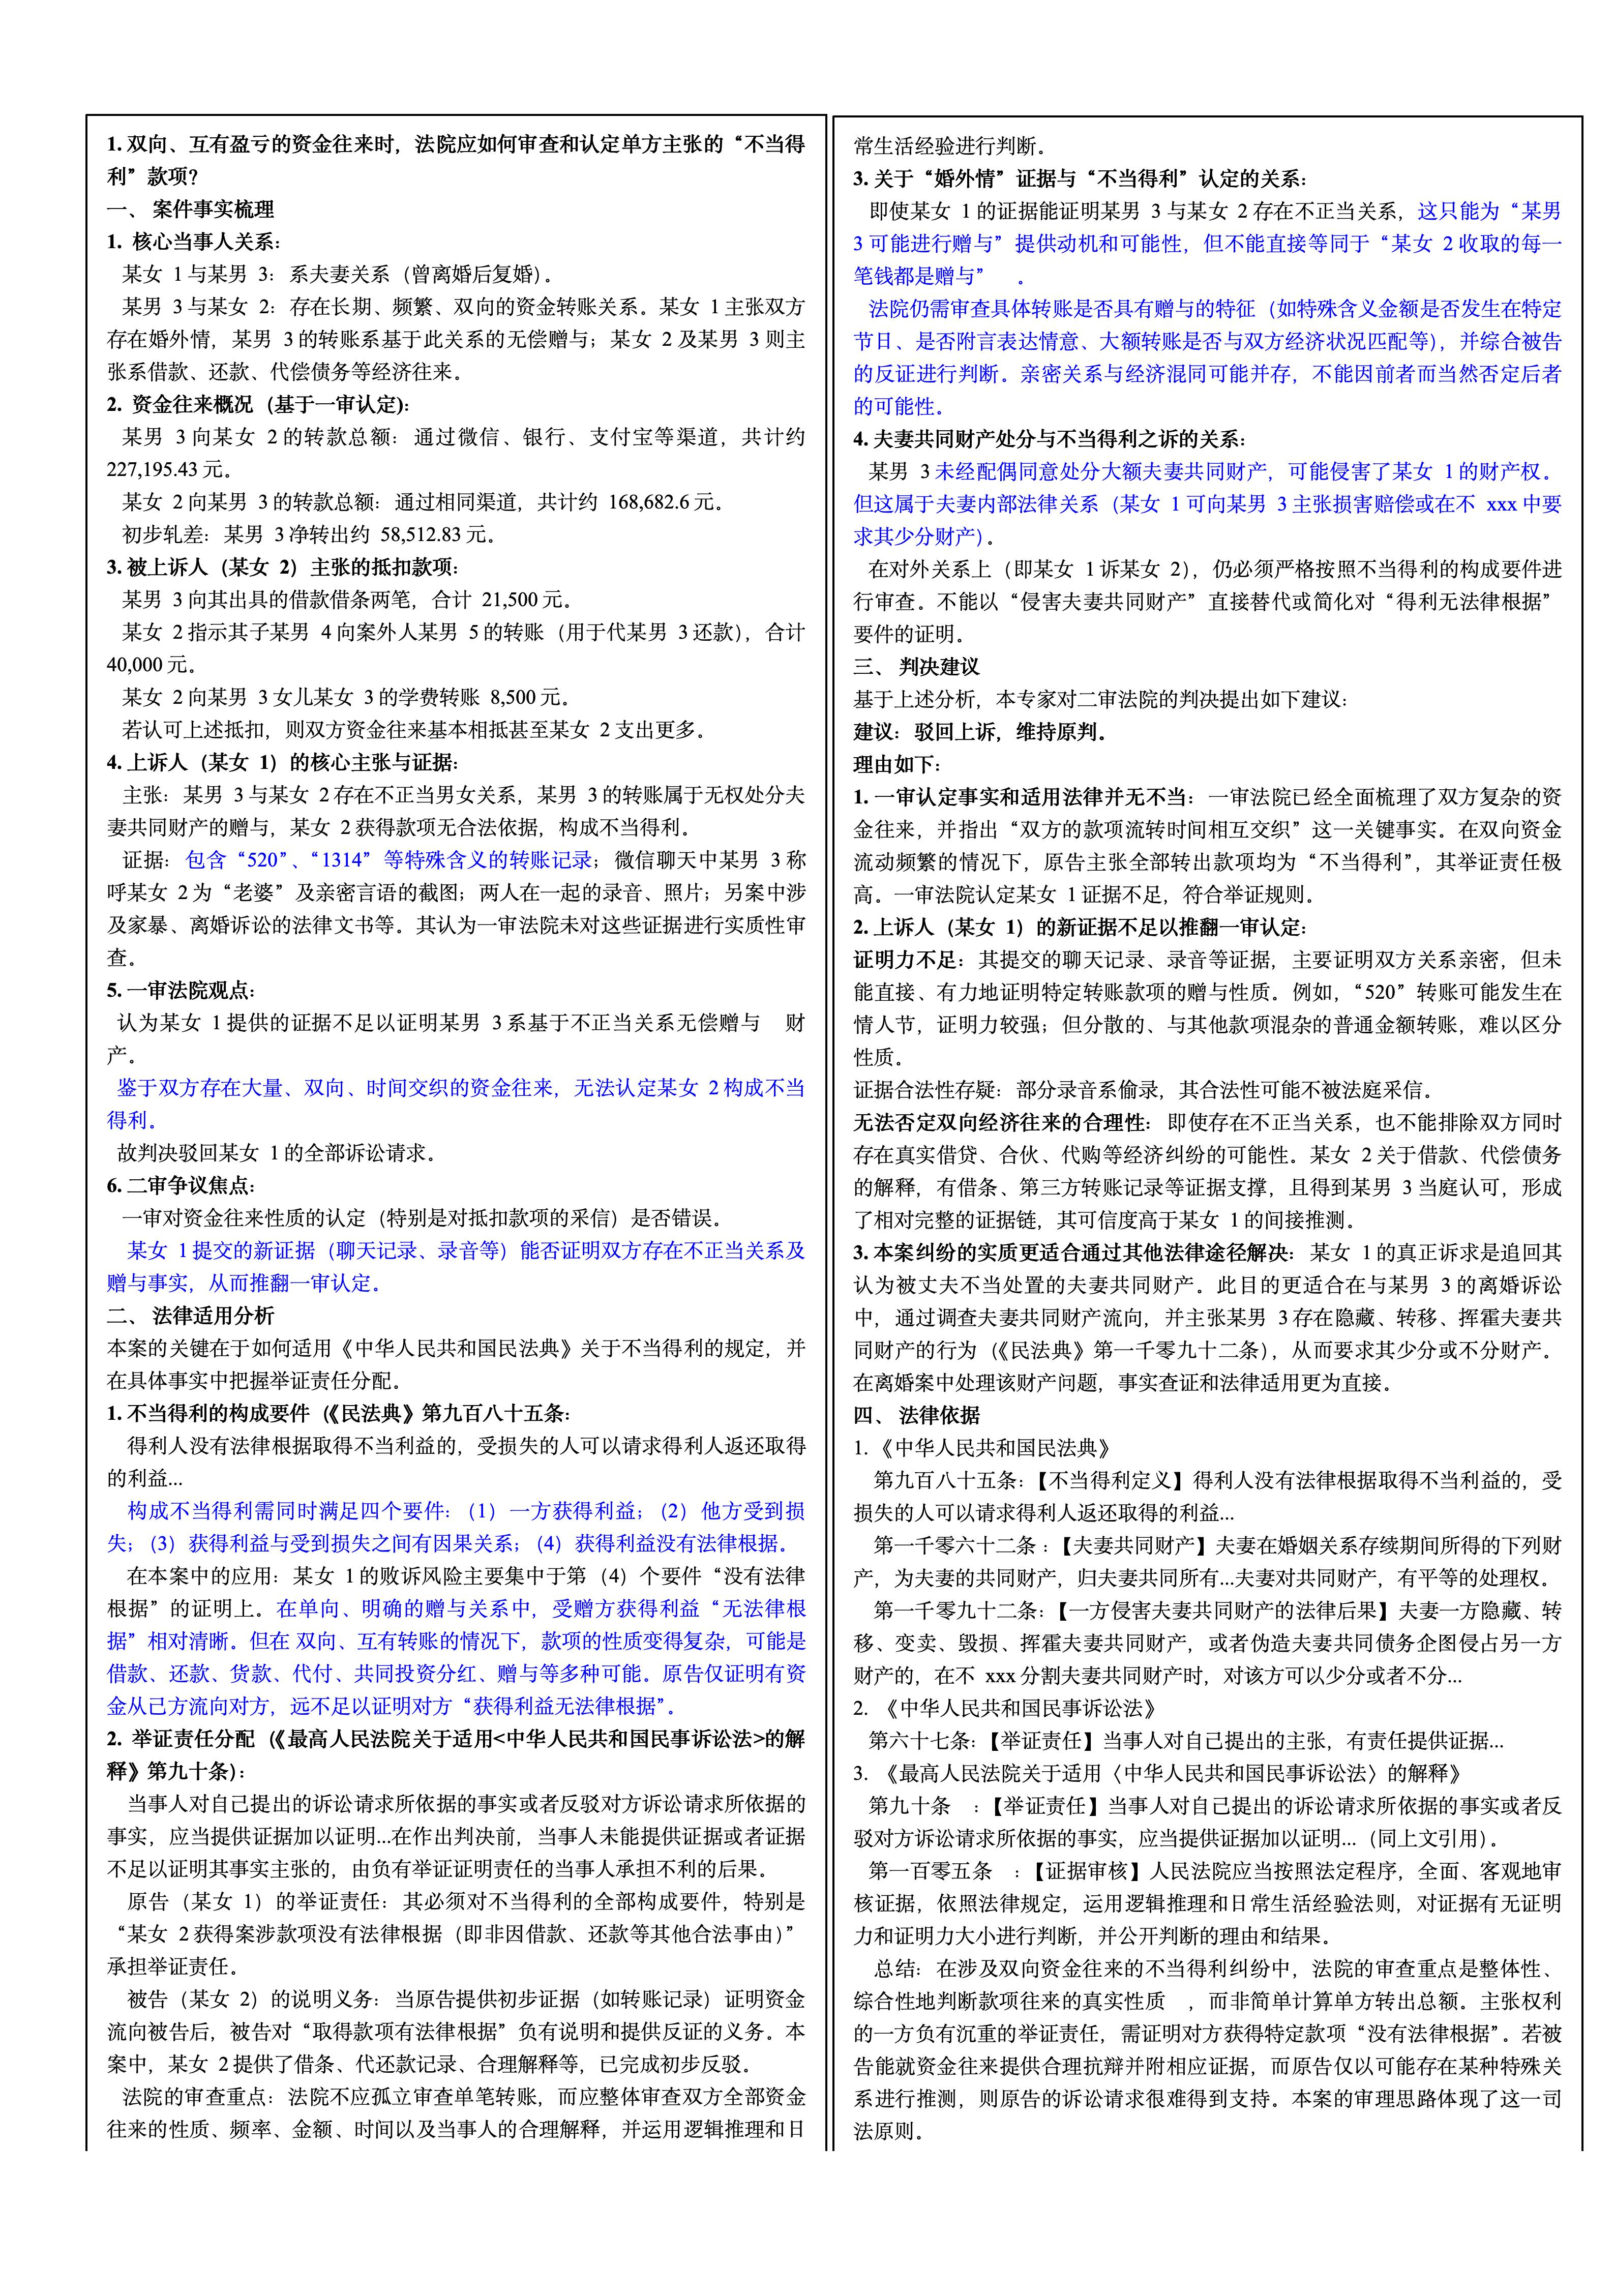
\includegraphics[width=\textwidth]{figures/media/Document1_01(1).jpg}
\caption{De-identified judgment segmentation and question-aligned summaries (sample 2).}
\label{fig:segmentation-cn-2}
\end{figure}

\end{appendices}

%%=============================================%%
%% For submissions to Nature Portfolio Journals %%
%% please use the heading ``Extended Data''.   %%
%%=============================================%%

%%=============================================================%%
%% Sample for another appendix section			       %%
%%=============================================================%%

%% \section{Example of another appendix section}\label{secA2}%
%% Appendices may be used for helpful, supporting or essential material that would otherwise 
%% clutter, break up or be distracting to the text. Appendices can consist of sections, figures, 
%% tables and equations etc.

% \end{appendices}

%%===========================================================================================%%
%% If you are submitting to one of the Nature Portfolio journals, using the eJP submission   %%
%% system, please include the references within the manuscript file itself. You may do this  %%
%% by copying the reference list from your .bbl file, paste it into the main manuscript .tex %%
%% file, and delete the associated \verb+\bibliography+ commands.                            %%
%%===========================================================================================%%
\clearpage
\bibliography{references_renumbered(1)}% author-year keys; use second bib file
%% if required, the content of .bbl file can be included here once bbl is generated
%%\input sn-article.bbl

\end{document}
